\chapter[Resultados]{Resultados en Bitcoin}{Resultados en Bitcoin}\label{Resultados}

\noindent
\rule{0.49\textwidth}{0.75pt} $_{\bigcirc}$ \rule{0.49\textwidth}{0.75pt}\\
Se mostró que las métricas de la blockchain pueden ayudar a mejorar la predicción del precio y que además con la metodología propuesta se logran alcanzar los mismos resultados que los métodos del estado del arte, por otro lado, aplicar TDA a series de tiempo volátiles ayuda a predecir cambios rápidos en la geometría de los datos pudiendo anticipar caídas graves en el precio, reflejándose esto en la clasificación para la toma de decisiones de inversión, con un modelo que puede asignar correctamente en un 95.76\% de los casos imagen a su respectivo agrupamiento de inversión.

\noindent
\rule{0.49\textwidth}{0.75pt} $_{\bigcirc}$ \rule{0.49\textwidth}{0.75pt}\\
\clearpage

\section{Resultados}
\label{subResultados}
Los resultados se mostraran en el orden en el que la metodología general debe ser llevada a cabo. Primero se obtienen las métricas que más influyen en la varianza del precio y que además están altamente correlacionadas con el mismo, después de obtener estas características son agregadas al conjunto de métricas financieras para ver el impacto en la predicción del precio, para ello los modelos son entrenados con distintas transformaciones matemáticas. Los resultados muestran una mejora de \$18 dólares frente a utilizar unicamente las características financieras. Luego se procede a obtener las normas topológicas del conjunto de datos totales y en un periodo de tiempo especifico, notando que esta norma es alta cuando se aproxima un crac financiero como los del 2018 o el 2021 por nombrar algunos. Por último estas características son agregadas a la entropía de Shannon calculada, a partir de las cuales se crean clusters de inversión. Se encontró que el modelo propuesto de clasificación para la toma de decisiones de inversión a mediano y largo plazo alcanza una exactitud del 95.76\%.

\section{Análisis de métricas}

\subsection{Datos y pre-procesamiento}
Después de cargar los métricas de la blockchain, introducir los datos faltantes y normalizar como se detalla en el \autoref{Metodologia}, al eliminar valores atípicos multivariados el conjunto de datos se reduce un 12\%  pasando de 3725 elementos a 3275.

En la \autoref{fig5} se observan las primeras cinco características de la blockchain después del pre-procesamiento.

\begin{figure}[!h]
	\centering
	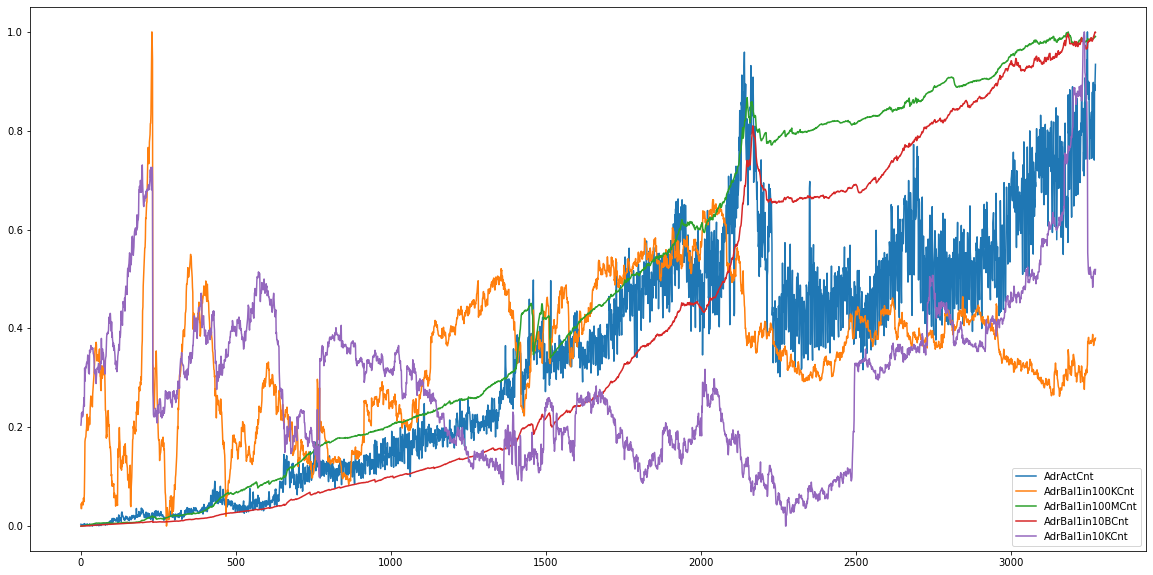
\includegraphics[scale=0.34]{Chapter5/metrics_1.png}
	\caption{Algunas métricas de la blockchain obtenidas para el análisis}
	\label{fig5}
\end{figure}

\subsection{Selección de métricas}

Antes de obtener los resultados del análisis de regresión hay que tratar con la multicolinealidad de los datos, siguiendo los pasos de \autoref{ssec:metrics} para el método VIF la correlación obtenida entre las métricas de la blockchain se muestra en la \autoref{fig6}, después de seleccionar aquellas que tuvieran una correlación mayor a $0.9$ como valor absoluto con al menos otra variable con el método de Pearson se obtuvo el subconjunto de características de la \autoref{fig7}. 

\begin{figure}[!h]
	\centering
	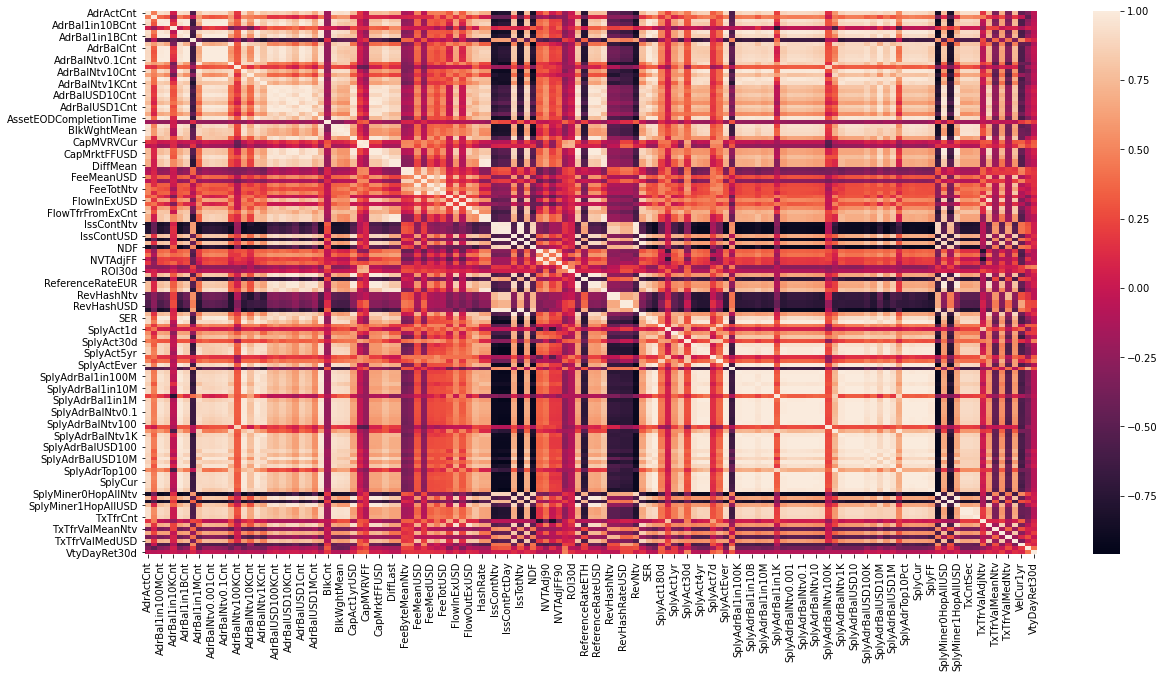
\includegraphics[scale=0.4]{Chapter5/corr_map.png}
	\caption{Correlación entre todas las métricas obtenidas}
	\label{fig6}
\end{figure}

\begin{figure}[!h]
	\centering
	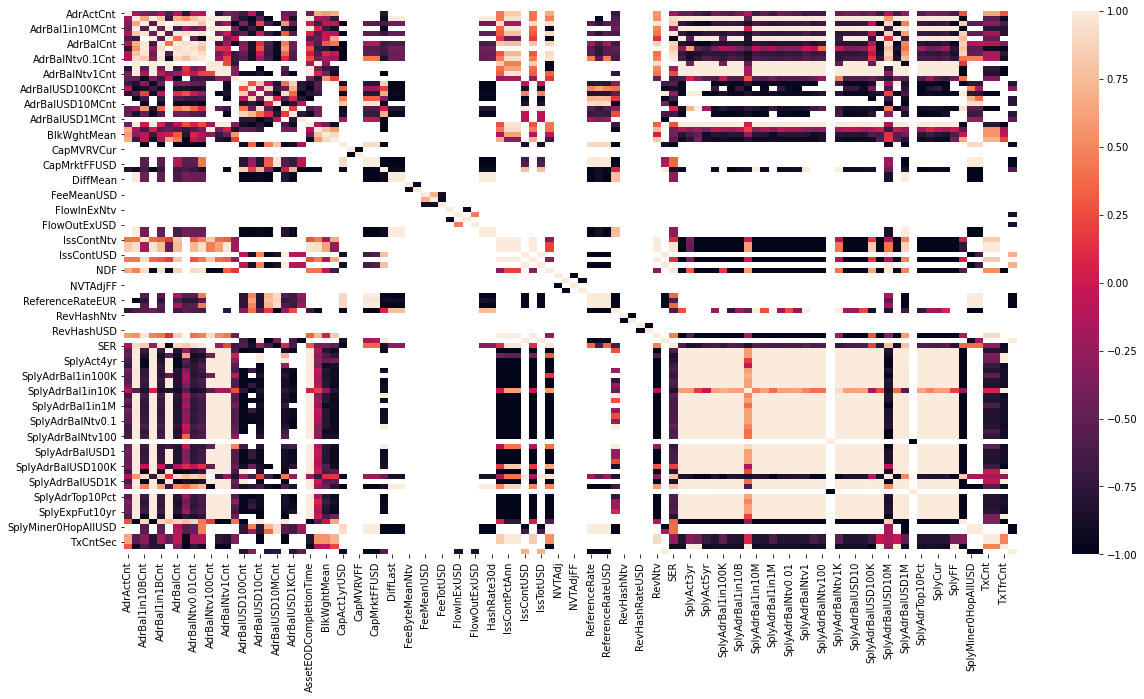
\includegraphics[scale=0.4]{Chapter5/corr_map2.png}
	\caption{Características de la blockchain con una correlación como valor absoluto mayor a 0.9}
	\label{fig7}
\end{figure}

Con las características obtenidas se calcula el VIF de las mismas como se muestra en la figura \autoref{subfig1}. La métrica con mayor multicolinealidad en los datos fue RevHashNtv mostrando mayor dependencia lineal en el supuesto de independencia. Esta variable es descartada y el VIF se calcula nuevamente. Se repite el proceso hasta obtener la tabla final de la figura \autoref{subfig2}, que son los datos a utilizar junto con aquellos que tienen poca correlación entre sí.

\begin{figure}[!h]
	\centering
	\subfloat[VIF con todas las métricas seleccionadas]
	{
		\label{subfig1}
		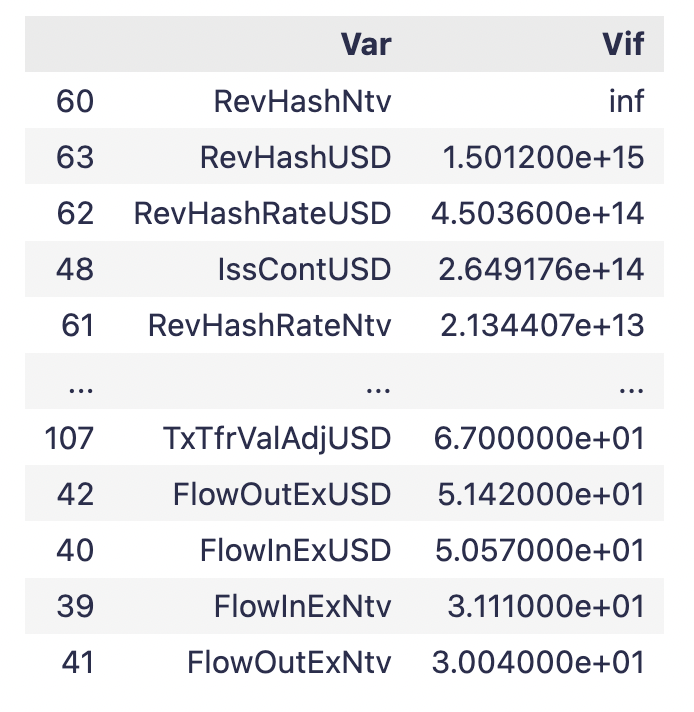
\includegraphics[width=0.45\columnwidth]{Chapter5/VIF.png}
	}
	\qquad
	\subfloat[Caracteristicas con VIF menor a cinco]
	{
		\label{subfig2}
		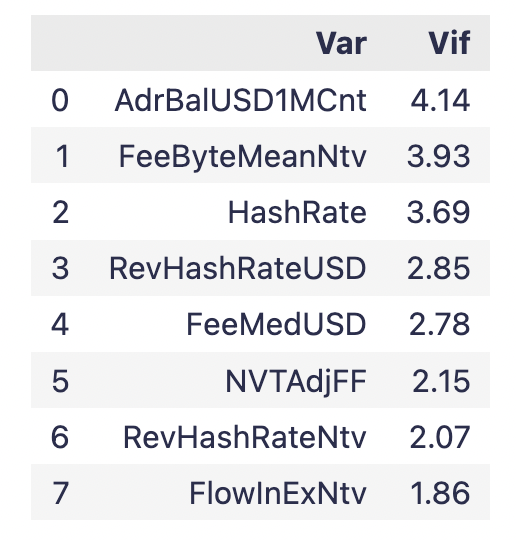
\includegraphics[width=0.45\columnwidth]{Chapter5/VIF2.png}
	}
	\caption{Tabla inicial y final después de aplicar el método VIF para eliminar multicolinealidad en los datos}
	\label{fig8}
\end{figure}

El análisis de regresión utilizando mínimos cuadrados ordinarios da la información mostrada en la \autoref{fig10}. Se puede ver que las variables con mayor peso en la predicción por el valor de sus coeficientes son \textit{AdrBalUSD1MCnt} y \textit{HashRate}.
Filtrando estas variables por su significación estadística se obtienen las características mostradas en la \autoref{fig11}. Estas variables son usadas en el análisis de componentes principales.


Los componentes principales de los datos con valores atípicos y sin valores atípicos se muestran en la \autoref{fig12} y \autoref{fig13} respectivamente. Se puede ver como hay una reducción en el número de puntos fuera del dominio de aplicabilidad (área verde), y como la gran mayoría de puntos se ajusta mejor dentro de los límites del mismo en los datos sin valores atípicos multivariados. El propósito del dominio de aplicabilidad es definir las fronteras donde el modelo puede ser utilizado y ofrecer predicciones confiables \parencite{karApplicabilityDomainStep2018}.

\begin{figure}
	\centering
	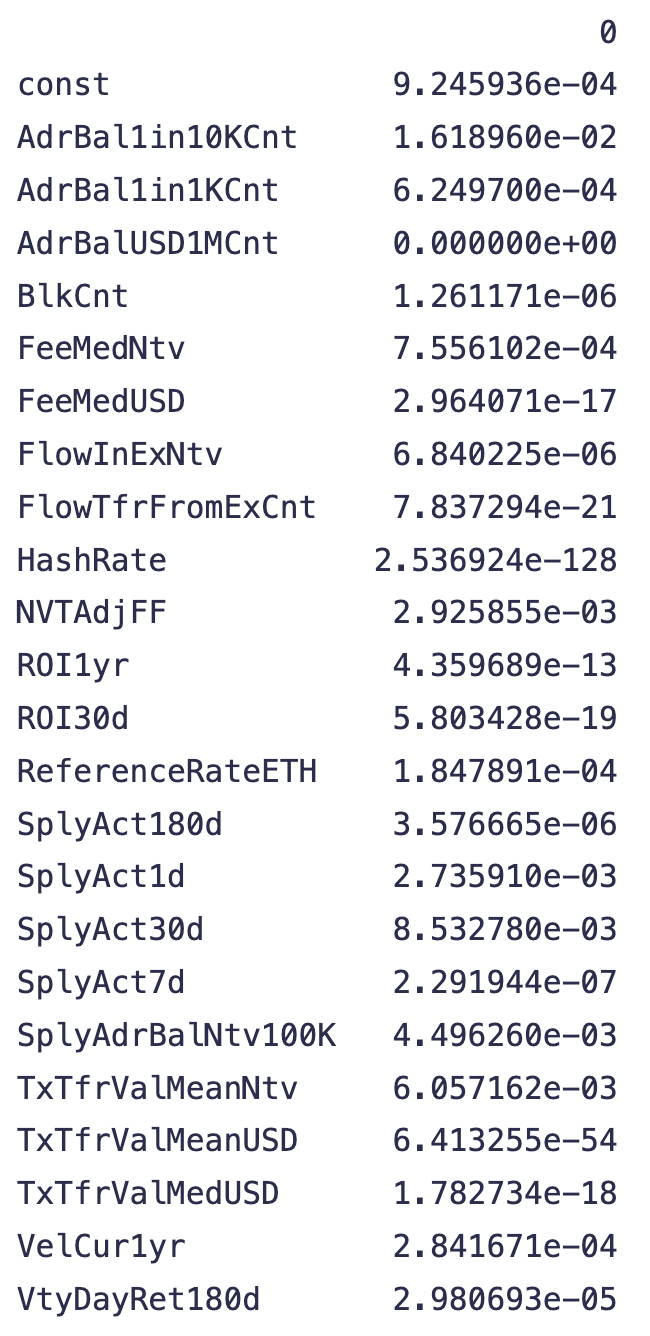
\includegraphics[scale=0.5]{Chapter5/p-val.png}
	\caption{Variables con valor p menor que 0.05}
	\label{fig11}
\end{figure}

\begin{figure}
	\centering
	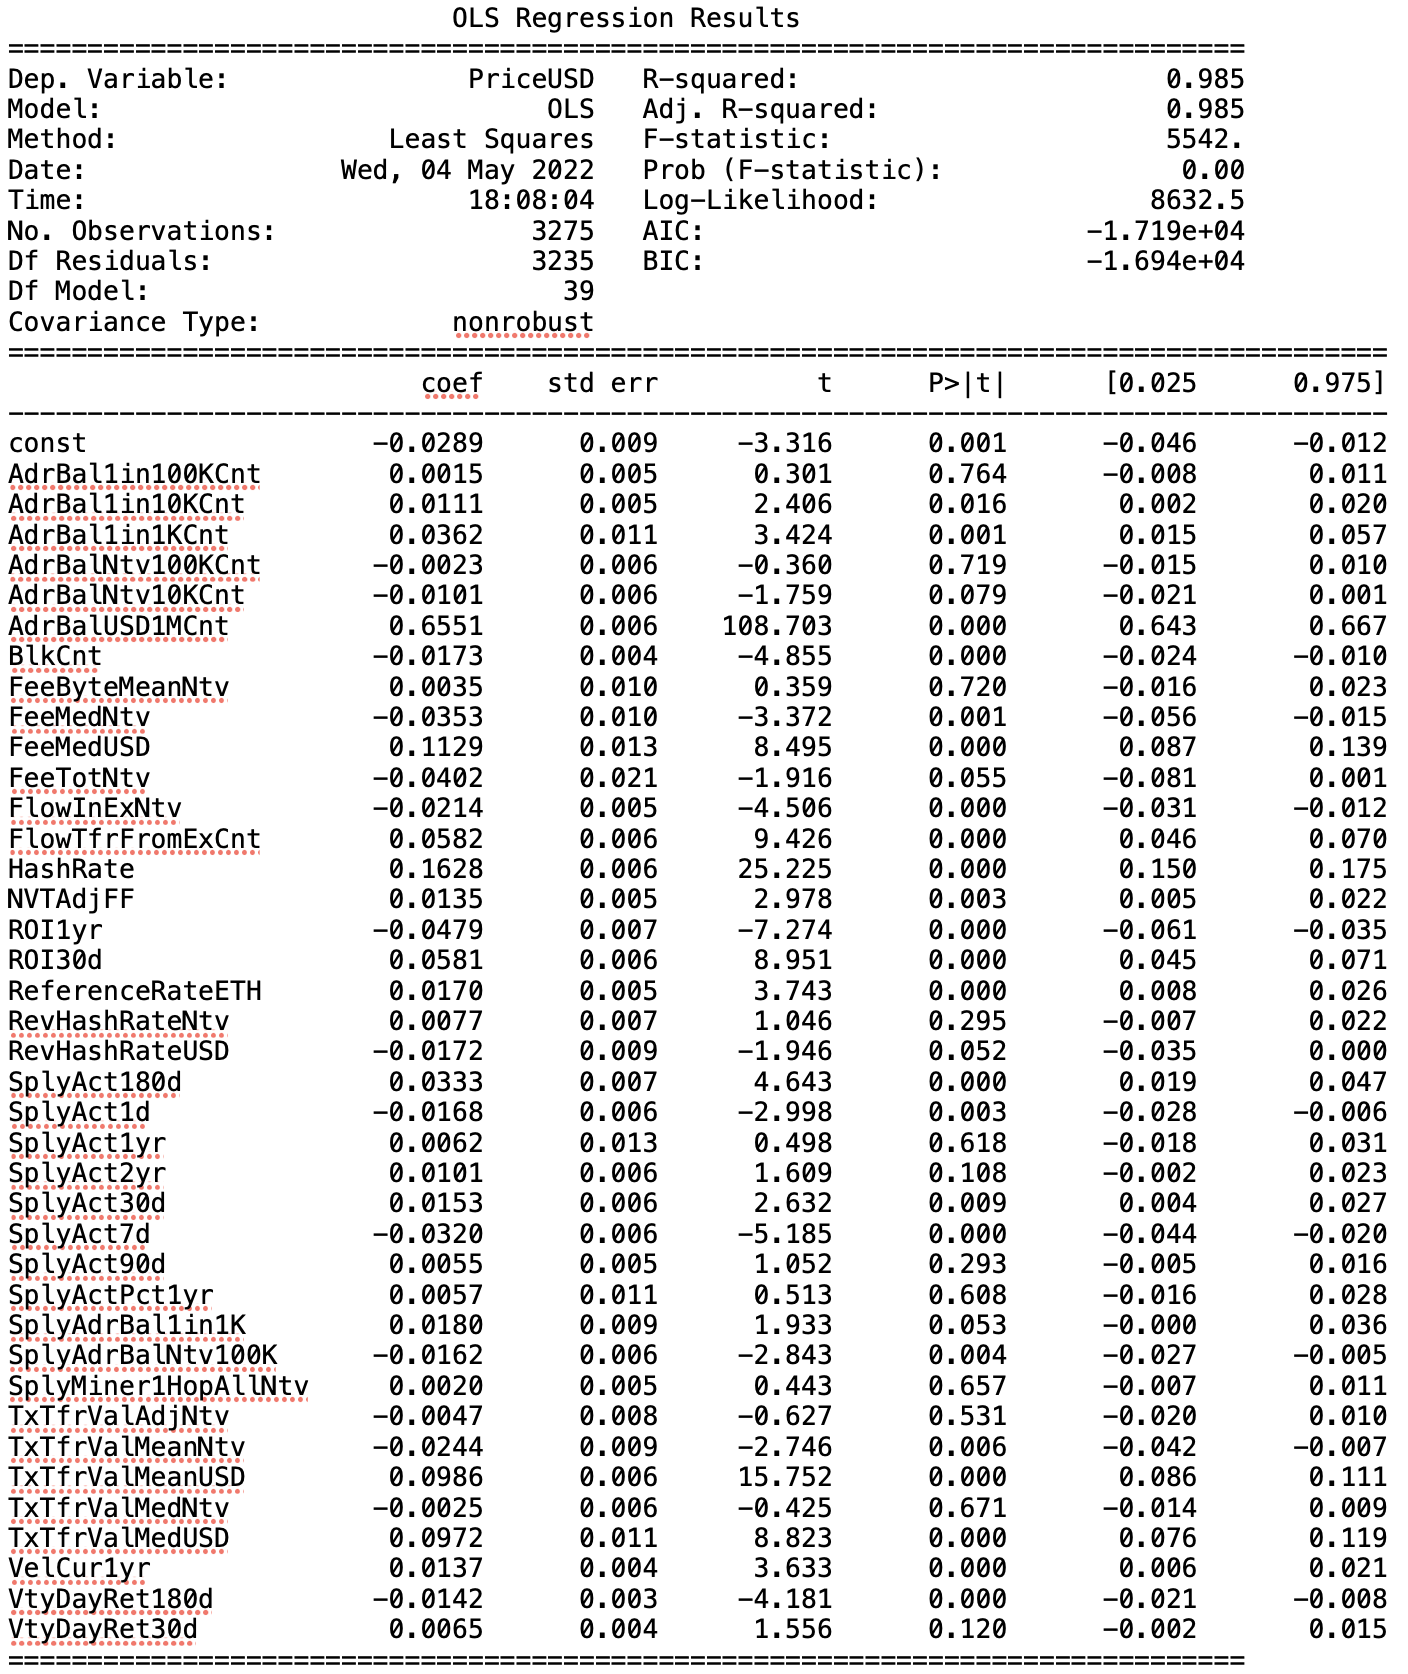
\includegraphics[scale=0.7]{Chapter5/OLS.png}
	\caption{Resultados del análisis de regresión}
	\label{fig10}
\end{figure}

\begin{figure}
	\centering
	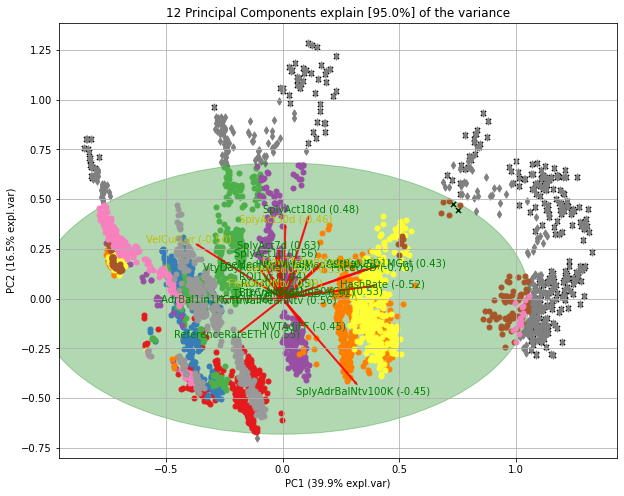
\includegraphics[scale=0.6]{Chapter5/pca_val_atipi.png}
	\caption{Componentes principales con valores atípicos multivariados}
	\label{fig12}
\end{figure}

\begin{figure}
	\centering
	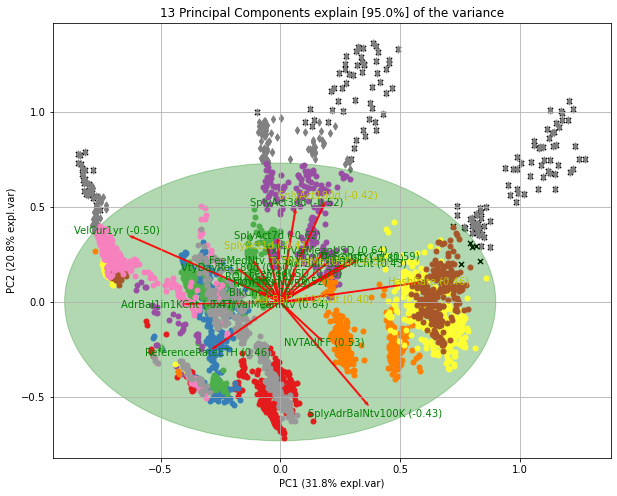
\includegraphics[scale=0.6]{Chapter5/pca_sin_va_atipi.png}
	\caption{Componentes principales sin valores atípicos multivariados}
	\label{fig13}
\end{figure}

Entonces, seleccionando aquellas variables que tienen la misma dirección y mayor o igual magnitud que el precio se obtienen los componentes principales de la \autoref{fig14}. Estas variables son: \textit{HashRate}, \textit{SplyAct180d} y \textit{SplyAct30d}. 

Realizando un dendrograma de correlación con las variables obtenidas se observa que el precio y hashrate pertenecen al mismo grupo, significando esto que es la variable que más afecta en la varianza del precio y que además está altamente correlacionada con el mismo. \textit{Hashrate} es la velocidad media a la que los mineros resuelven hashes durante el día. La velocidad del hash es la velocidad a la que se completan los cálculos de todos los mineros de la red. Esta velocidad se deriva de la dificultad de minado y de la velocidad en la que el bloque fue emitido. 

\begin{figure}
	\centering
	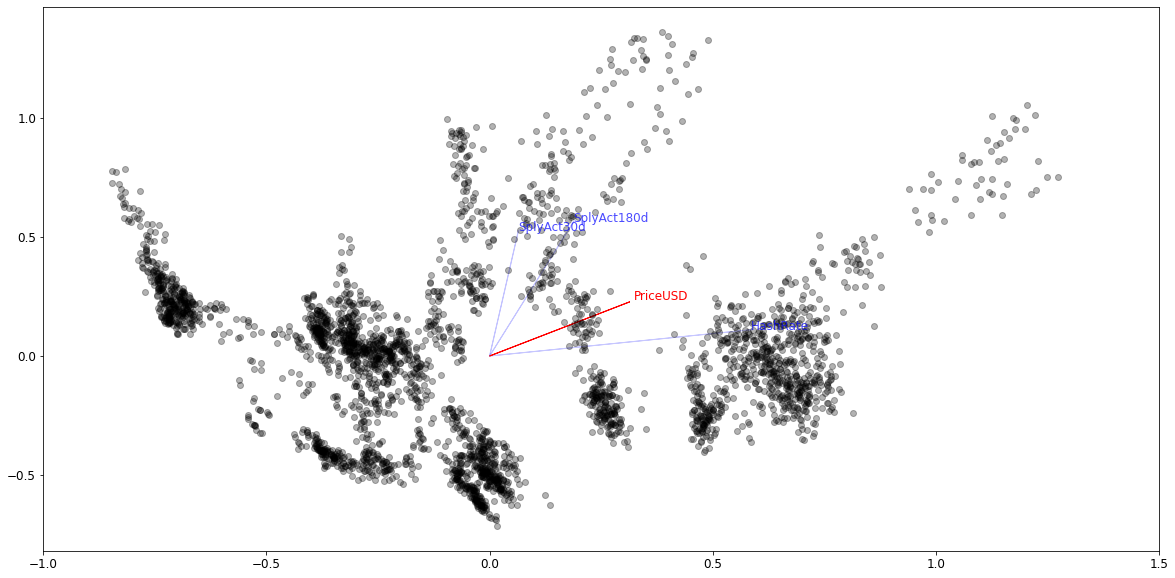
\includegraphics[scale=0.4]{Chapter5/pca_price.png}
	\caption{Métricas obtenidas que influye en la varianza del precio}
	\label{fig14}
\end{figure}

\begin{figure}
	\centering
	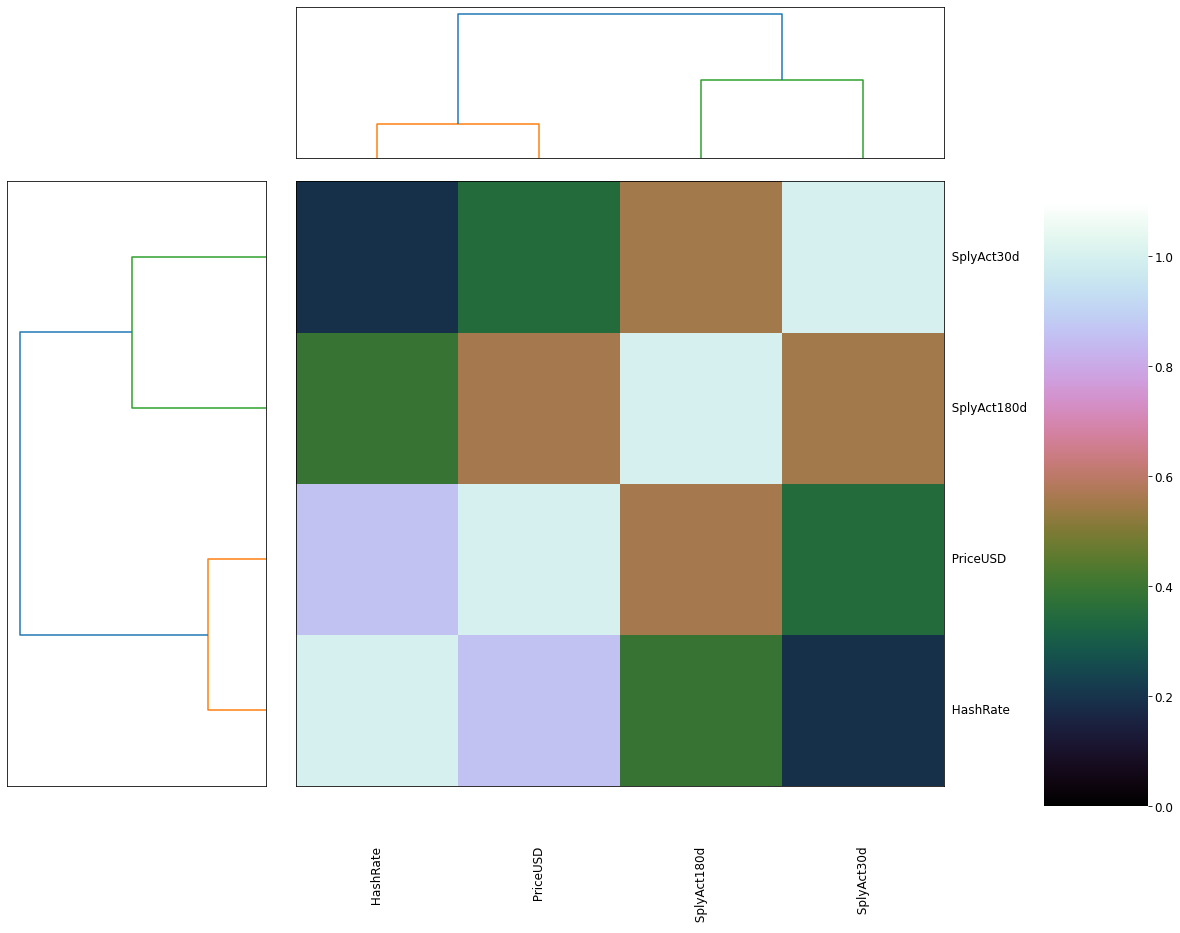
\includegraphics[scale=0.3]{Chapter5/dendo.png}
	\caption{Dendrograma de correlación con las métricas obtenidas por el PCA}
	\label{fig15}
\end{figure}

\section{Predicción del precio}

\subsection{Datos y pre-procesamiento}
Los datos descargados y procesados en formato OHLCV tienen la estructura mostrada en \autoref{fig16}, después de realizar el análisis de métricas de la blockchain detallado en la \autoref{Metodologia} se llega al conjunto de datos final mostrado en la \autoref{fig17}.

\begin{figure}[h!]
	\centering
	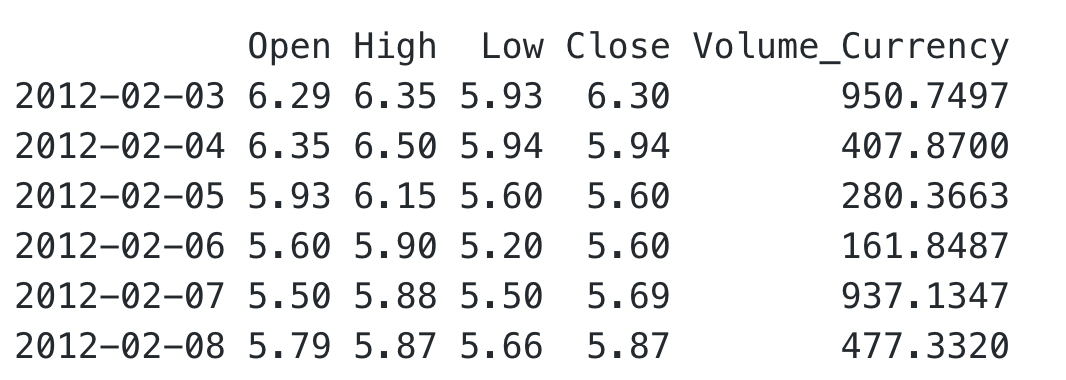
\includegraphics[scale=0.5]{Chapter5/ohlcv.png}
	\caption{Características financieras en formato OHLCV}
	\label{fig16}
\end{figure}

\begin{figure}[h!]
	\centering
	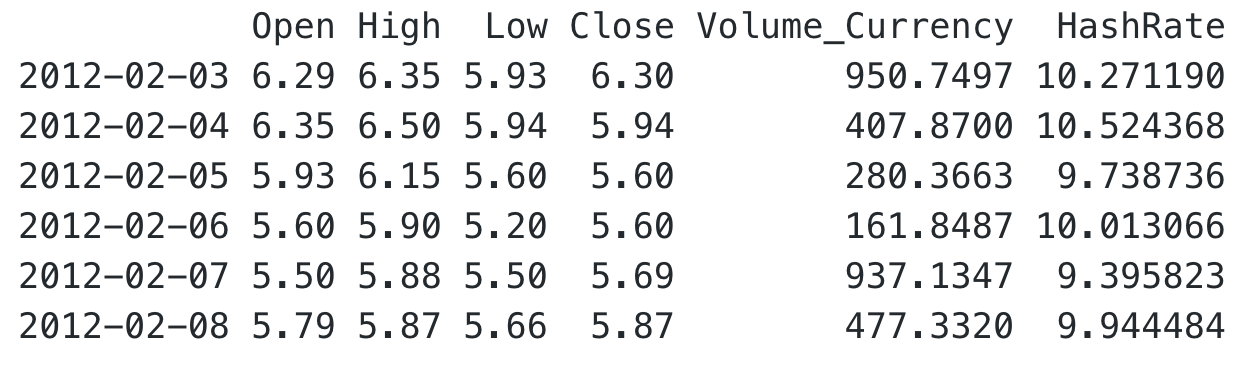
\includegraphics[scale=0.5]{Chapter5/ohlcv_complete.png}
	\caption{Conjunto de datos final con la métrica obtenida por el análisis de la blockchain}
	\label{fig17}
\end{figure}

La volatilidad del precio de cierre del activo se muestra en la \autoref{fig18}. En esta se puede ver como a partir del 2017 el precio empieza a despegar de forma exponencial, llegando a valer en 2018 casi \$20,000 dólares y a su vez ocurriendo su primer crac debido a la salida y poco apoyo de grandes financieros como Goldman Sachs o a la división de la comunidad creando un fork con una nueva visión de la moneda \parencite{peterssonWhyBitcoinCrashed2018}. Sea como fuere, la criptomoneda comenzó una etapa lenta de recuperación con caídas de por medio como la de 2019 o 2020 debido a sanciones de grandes países como China, aun así, desde finales de 2020 el precio ha vuelto a su crecimiento exponencial debido a la aceptación de cada vez más empresas y el público en general pero manteniendo su gran volatilidad. Actualmente, a inicios de mayo de 2022, el precio ronda aproximadamente los \$40,000 dólares manteniendo cierta estabilidad a pesar de la crisis económica causada por la COVID-19 y la invasión de Rusia a Ucrania.

\begin{figure}[h!]
	\centering
	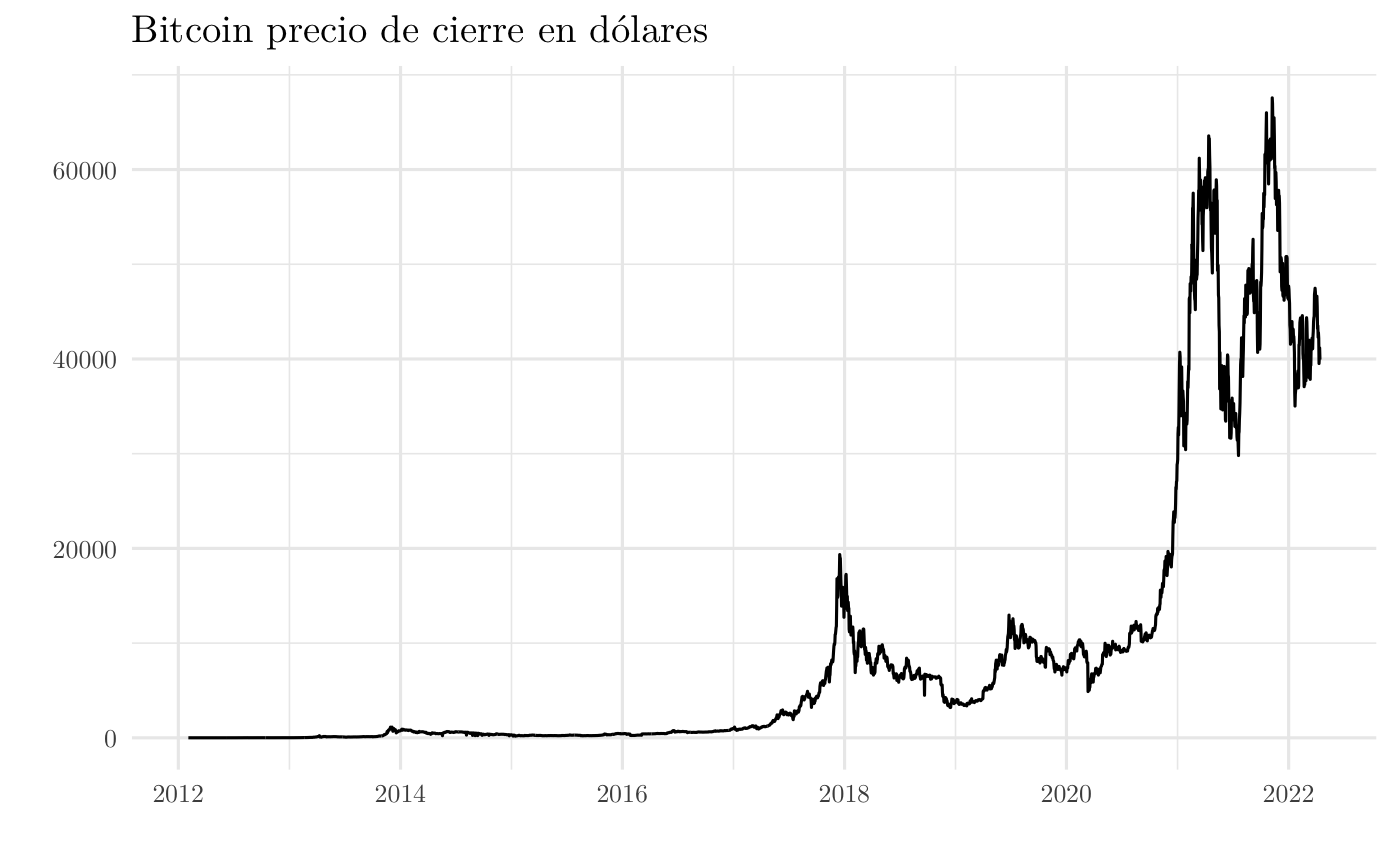
\includegraphics[scale=0.35]{Chapter5/btc_price.png}
	\caption{Serie de tiempo del precio del bitcoin en dólares}
	\label{fig18}
\end{figure}

\subsection{Selección de modelo}

La correlación entre las variables financieras se muestra en la \autoref{fig19}, donde se puede observar que todas las características cuentan con una correlación muy alta y por lo tanto todas son tomadas en cuenta para el análisis de precio. Estas variables son transformadas como se muestra en la \autoref{met:prediccion}. Los resultados se pueden observar en la \autoref{fig20}. 

\begin{figure}[h!]
	\centering
	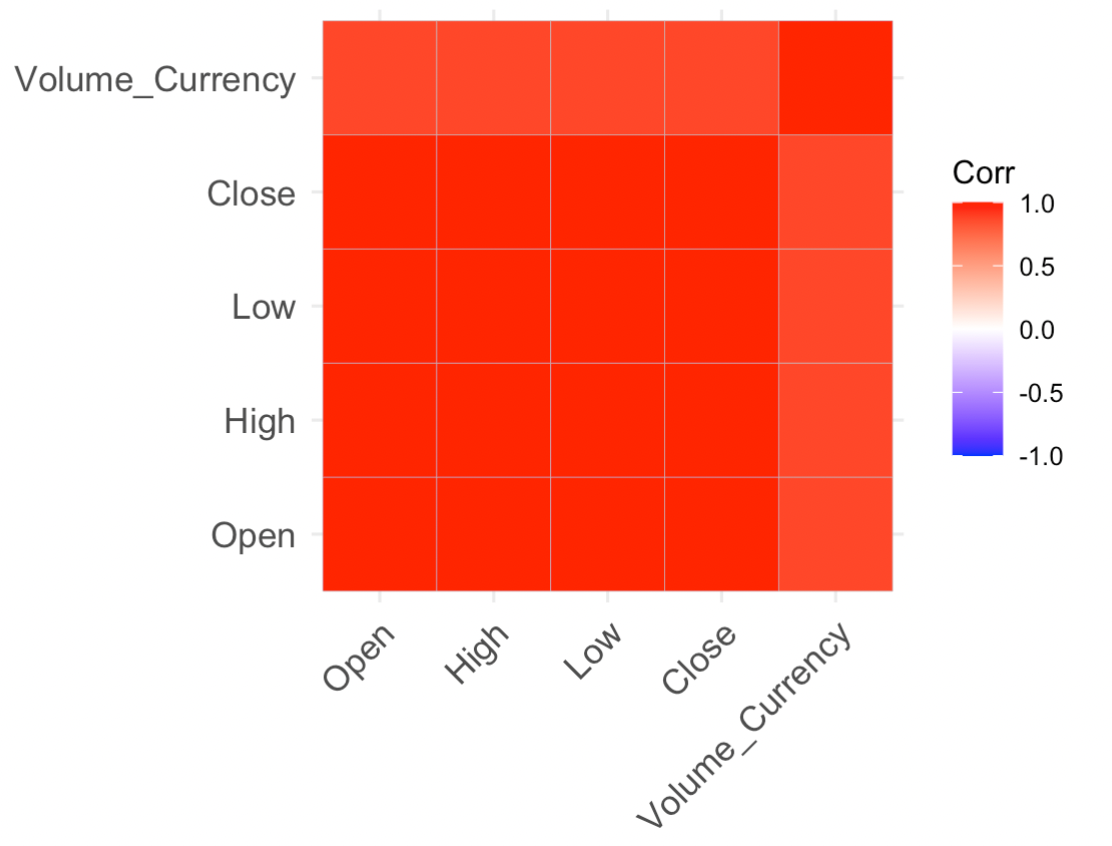
\includegraphics[scale=0.5]{Chapter5/finance_corr.png}
	\caption{Correlación entre métricas financieras}
	\label{fig19}
\end{figure}

\begin{figure}[!h]
	\centering
	\subfloat[Transformación logaritmica]
	{
		\label{subfig3}
		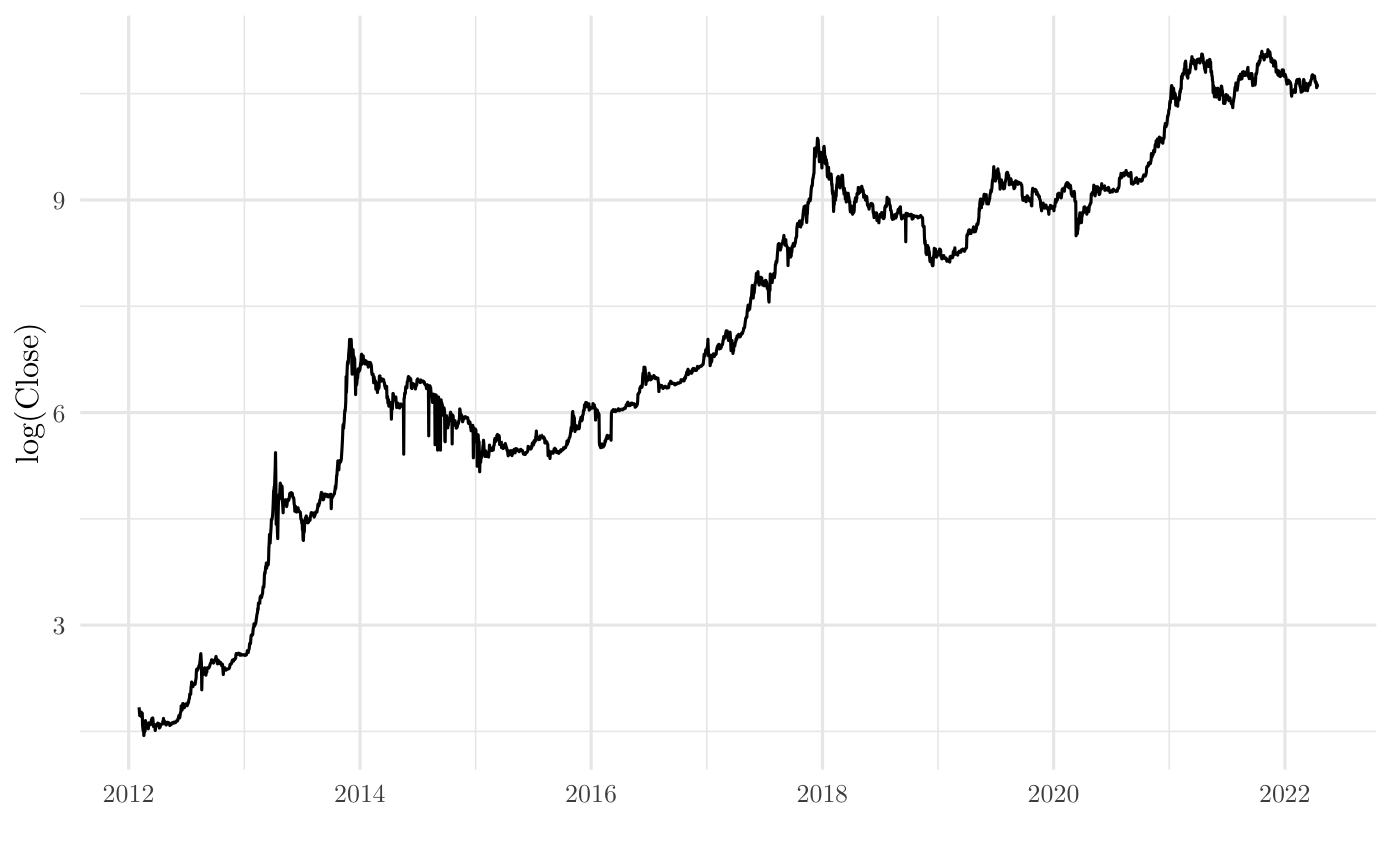
\includegraphics[width=0.45\columnwidth]{Chapter5/log_close.png}
	}
	\qquad
	\subfloat[Transformación BoxCox]
	{
		\label{subfig4}
		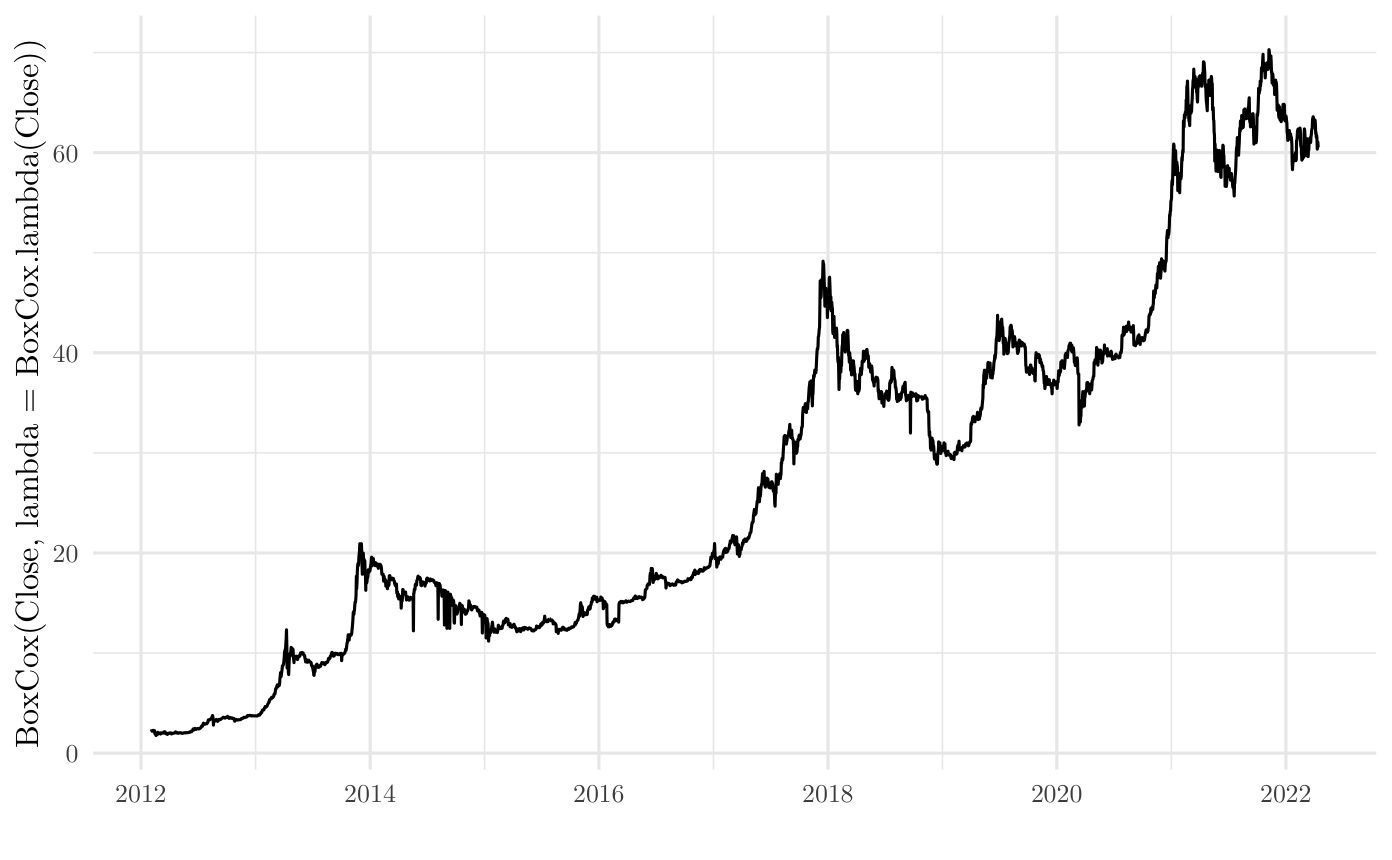
\includegraphics[width=0.45\columnwidth]{Chapter5/boxcox_close.png}
	}
	\qquad
	\subfloat[Retornos diarios del precio]
	{
		\label{subfig5}
		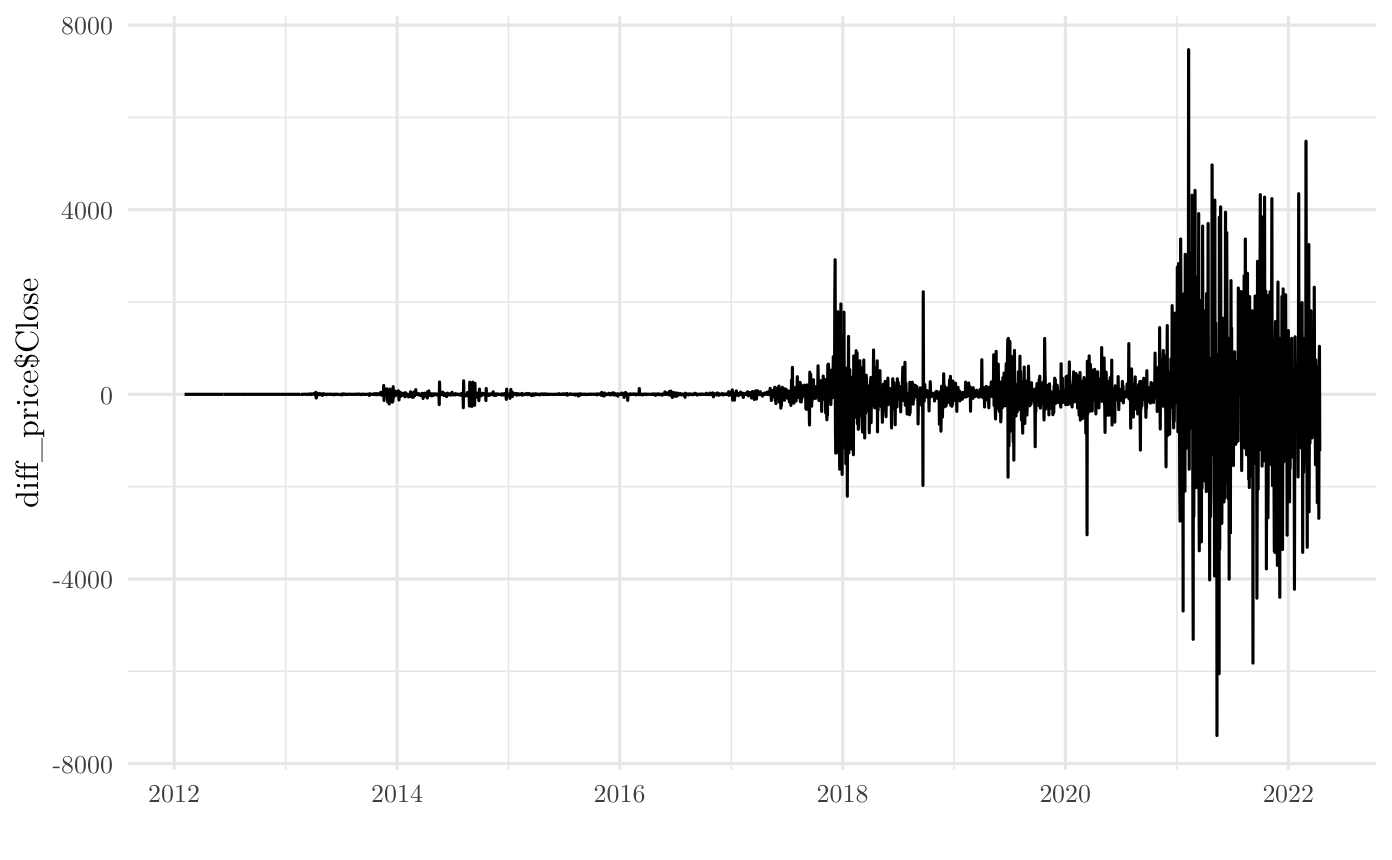
\includegraphics[width=0.45\columnwidth]{Chapter5/diff_close.png}
	}
	\qquad
	\subfloat[Retornos logaritmicos del precio]
	{
		\label{subfig6}
		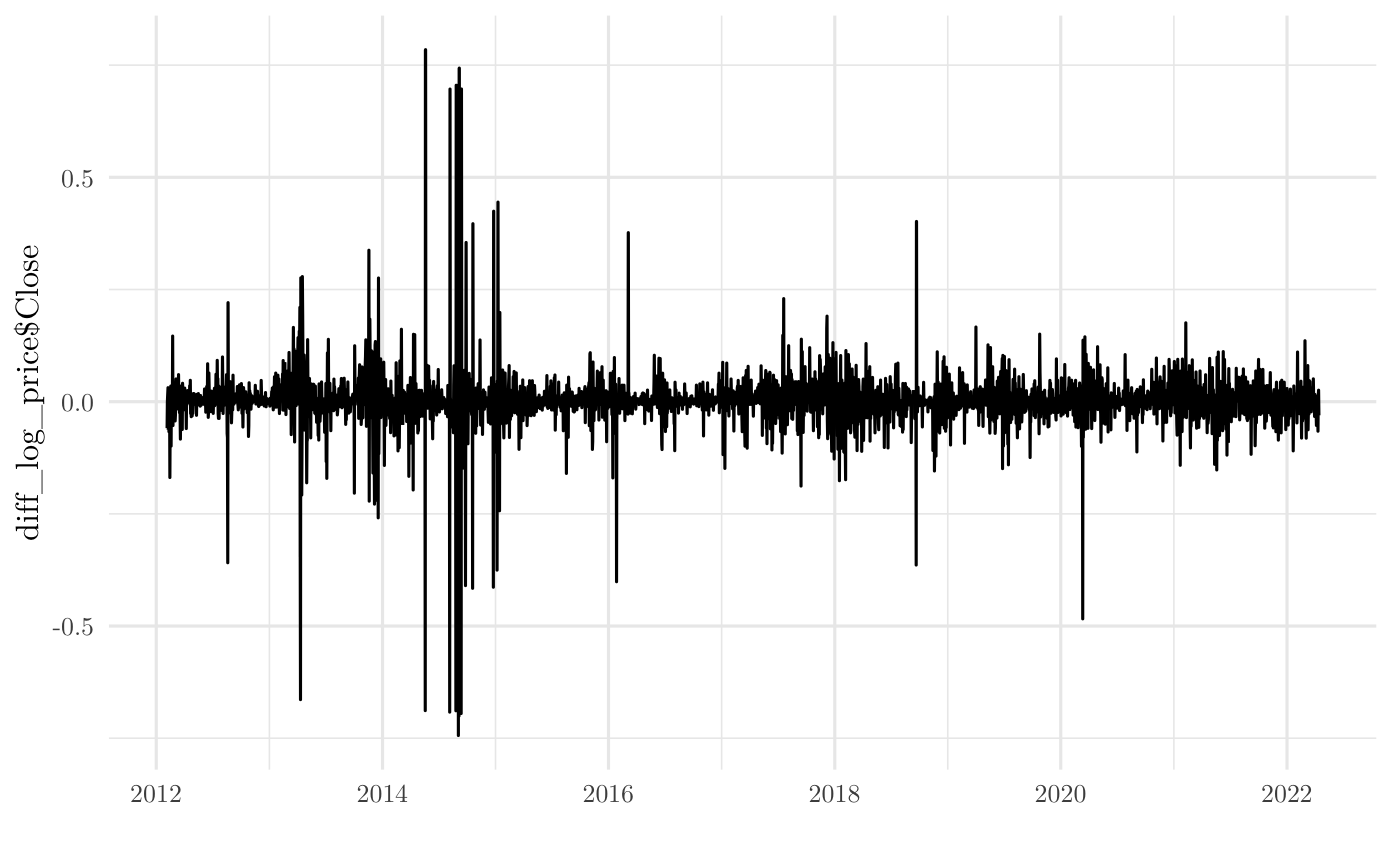
\includegraphics[width=0.45\columnwidth]{Chapter5/diff_log_price.png}
	}
	\caption{Transformaciones matemáticas aplicadas a los datos}
	\label{fig20}
\end{figure}

El parámetro lambda encontrado que mejor estabiliza la varianza en la transformación BoxCox es $\lambda = 0.2689427$, aunque la transformación logaritmica muestra una mejor tendencia a simple vista, por otro lado, las diferencias del precio muestran que en los últimos años han habido mayores rendimientos, sin embargo, si la comparamos con las diferencias logarítmicas el porcentaje de rendimientos no es mayor que el de finales del 2014. 

Después de entrenar los datos transformados con los distintos modelos seleccionados y calculando sus indicadores de error y exactitud, se elabora la \autoref{tab:Table4}. Se observa que el modelo con el menor indice de error y exactitud es Random Forest alcanzando un error de \$38.63 dólares.
En la \autoref{fig21} se pude ver la predicción sobre el conjunto de datos de prueba, los puntos negros son los datos originales y la linea roja los datos predichos. Si se realiza el mismo ejercicio sobre únicamente las características financieras con el modelo RF se alcanza un error de \$56.77 dólares, mostrándose que agregando esta única característica puede mejorar la predicción hasta \$18.14 dólares.
 
\begin{table}
	\centering
	\begin{adjustbox}{width=0.83\textwidth}
	\begin{tabular}{m{5cm} m{3.5cm} m{3cm} m{3cm} }
		\toprule
		\textbf{Transformación} & \textbf{Modelo} & \textbf{RMSE} & \textbf{Theil’s U}\\
		\midrule
		Original&Naive & 237.2850  & 0.05137089\\
		&SES   & 237.2542  & 0.05136421\\
		&Holt  & 237.2228  & 0.05135741\\
		&ETS   & 255.9911  & 0.05542065\\
		&ARIMA & 237.2850  & 0.05137089\\
		&RTS   & 82.86021   & 0.01793877\\
		&SVM   & 142.1834   & 0.03078192\\
		&RF    & \textbf{39.38410}   & \textbf{0.00852643}\\
		&LSTM  & 1.40e+07  & 3049.5840\\ \\
		log	&Naive & 2.372850  & 0.05137089\\
		&SES   & 246.9256  & 0.05345801\\
		&Holt  & 247.6223  & 0.05360884\\
		&ETS   & 247.6223  & 0.05360884\\
		&ARIMA & 247.7399 & 0.05363431\\
		&RTS   & 89.22367   & 0.01931643\\
		&SVM   & 385.0302   & 0.08335690\\
		&RF    & \textbf{38.62311}   & \textbf{0.00836168}\\
		&LSTM  & 2.74e+14  & 5.938e+10\\ \\
		BoxCox	&Naive & 2.372850  & 0.05137089\\
		&SES   & 242.2361  & 0.05244277\\
		&Holt  & 242.3319  & 0.05246350\\
		&ETS   & 250.4998  & 0.05423181\\
		&ARIMA & 242.7126 & 0.05254592\\
		&RTS   & 85.04896   & 0.01841263\\
		&SVM   & 183.3686   & 0.03969827\\
		&RF    & \textbf{38.73046}   & \textbf{0.00838493}\\
		&LSTM  & 2.43e+09  & 52683.350\\ \\
		diff		&Naive & 336.2168  	& 0.07278906\\
		&SES   & 237.2766  	& 0.05136907\\
		&Holt  & 237.2176  	& 0.05135629\\
		&ETS   & 237.2766 	& 0.05136907\\
		&ARIMA & 237.2852  	& 0.05137092\\
		&RTS   & 317.0049   & 0.06862979\\
		&SVM   & 328.3989   & 0.07109653\\
		&RF    & 320.6893	& 0.06942740\\
		&LSTM  & 27824.87  	& 6.02393013\\ \\
		diff(log)	&Naive & 237.2976  	& 0.05137361\\
		&SES   & 237.2964  	& 0.05137335\\
		&Holt  & 237.2964  	& 0.05137335\\
		&ETS   & 237.2964  	& 0.05137335\\
		&ARIMA & 237.2960 	& 0.05137327\\
		&RTS   & 237.2942  	& 0.05137287\\
		&SVM   & 237.2944  	& 0.05137291\\
		&RF    & 237.2939  	& 0.05137281\\
		&LSTM  & 237.2968	& 0.05137345\\
		\bottomrule
		\hline
	\end{tabular}
	\end{adjustbox}
	\caption{Resultados de la comparación de los modelos durante la fase de entrenamiento estimando RMSE y Theil’s U.}
	\label{tab:Table4}
\end{table}  
\section{Análisis topológico de datos}

\begin{figure}
	\centering
	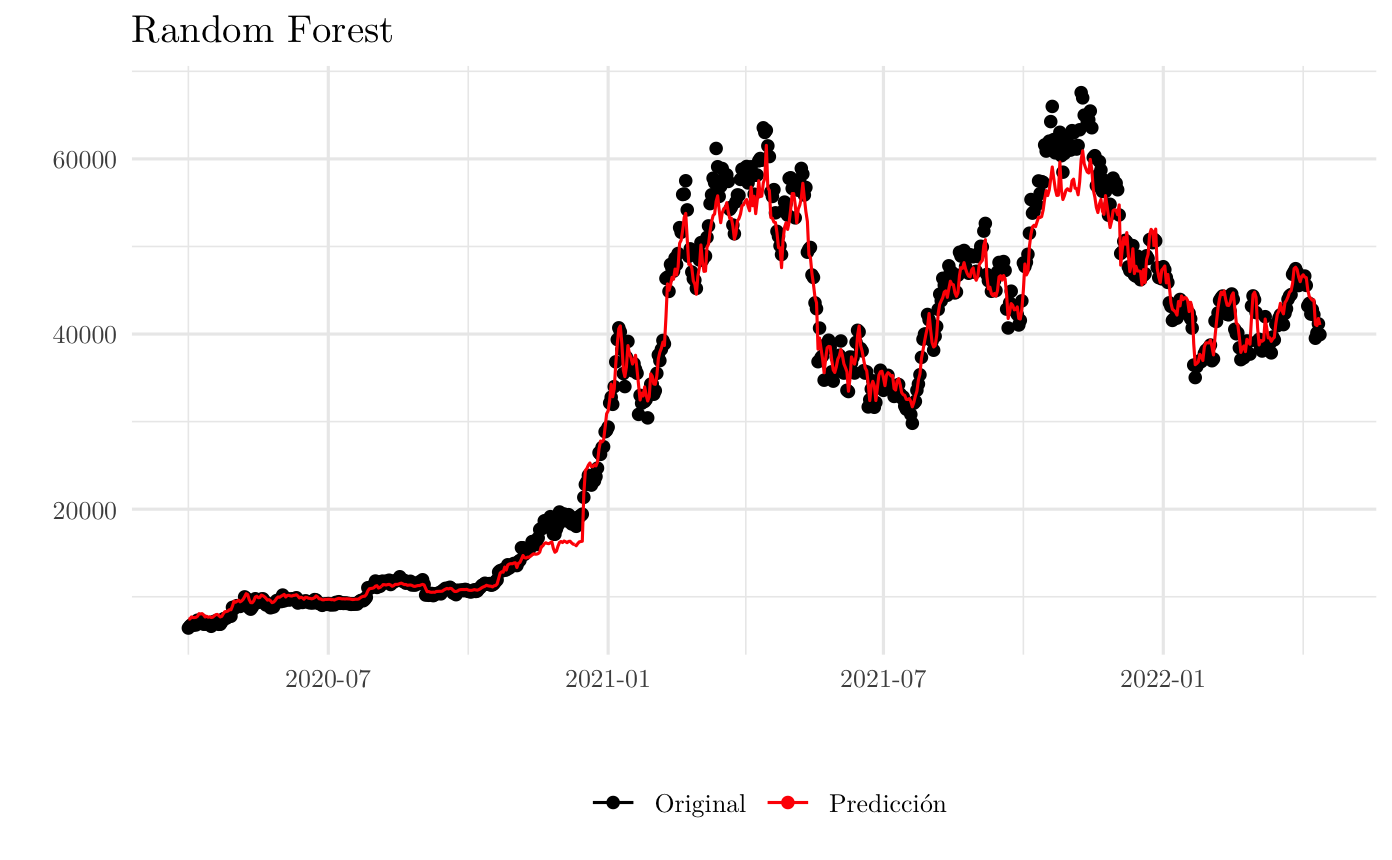
\includegraphics[scale=0.35]{Chapter5/pred_RF.png}
	\caption{Predicción sobre el conjunto de prueba}
	\label{fig21}
\end{figure}

\subsection{Norma $C^1$}

Para encontrar un crac en un periodo de tiempo especifico se recomienda segmentar la serie de tiempo en intervalos pequeños que inicien y terminen en las correspondientes caídas críticas \parencite{gideaTopologicalRecognitionCritical2020}, sin embargo, para la toma de decisiones de inversión se intentó capturar la mayor cantidad de caídas en todo el periodo establecido. Después de aplicar la metodología de la \autoref{met_tda} se obtuvieron los normas $L^1$ de los panoramas de persistencia de las nubes de datos generados con una ventana deslizante de 50 días como recomienda Guidea y col. \parencite*{gideaTopologicalRecognitionCritical2020} en su artículo. La \autoref{fig22} muestra los cambios en la forma de los datos en periodos de tiempo específicos, entonces, antes de una transición crítica los valores absolutos de las diferencias también toman valores cada vez más altos, siendo la suma de estos la norma $C^1$, que tiene la ventaja de crecer mucho en un instante de tiempo previo al actual si se acerca a un cambio rápido en la geometría de los datos. La \autoref{fig23} nos muestra los resultados de aplicar TDA al precio de cierre del bitcoin y calcular la norma $C^1$. La explicación de los picos máximos y su relación con las caídas más pronunciadas en el precio se detallaran más adelante en la \autoref{res_clasificacion}.

\begin{figure}
	\centering
	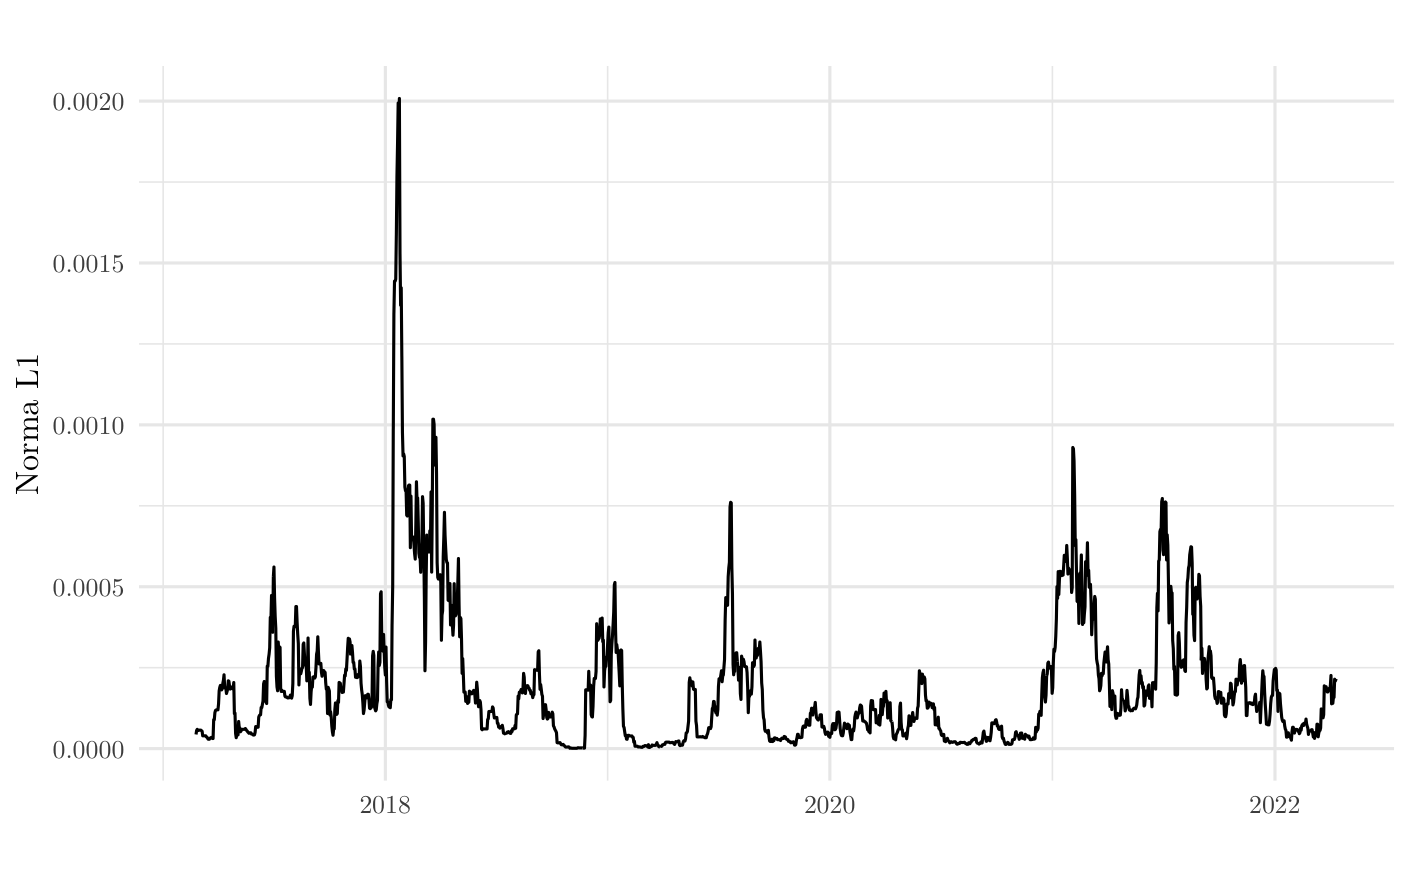
\includegraphics[scale=0.3]{Chapter5/norm_l1.png}
	\caption{Norma $L^1$ de los datos totales}
	\label{fig22}
\end{figure}

\begin{figure}
	\centering
	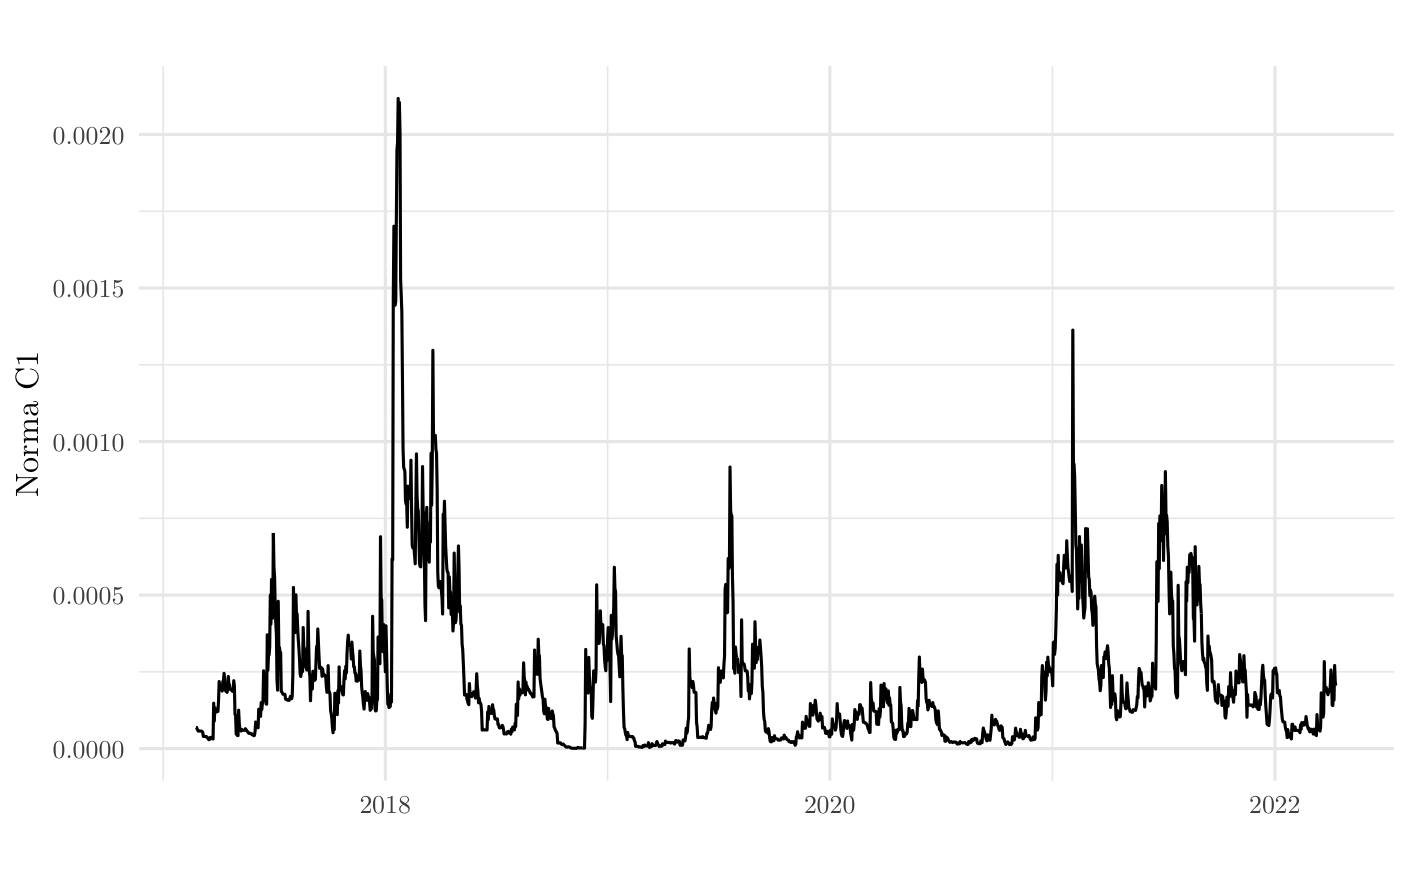
\includegraphics[scale=0.3]{Chapter5/norm_c1.png}
	\caption{Norma $C^1$ de los datos totales}
	\label{fig23}
\end{figure}

\subsection{Cluster de riesgo}

Tomando ventaja de la metodología para la detección de cracs económicos se estudian los últimos 90 días del la serie de tiempo del precio y se realiza un análisis de caídas, para ello primero se cargan los datos de los últimos tres meses y se calcula la norma $C^1$ de los datos como se muestra en la \autoref{fig24}, luego se calculan los posibles clusters de riesgo usando K-means como se explica en la \autoref{met_tda} y se selecciona el agrupamiento según los criterios antes especificados en la metodología. En este caso se obtuvieron los clusters de la \autoref{fig25} donde se puede deducir que el cluster de riesgo es el uno y se comprueba colocando el agrupamiento sobre los datos originales como en la \autoref{fig26}. Esto se realiza de forma automática y será de ayuda para complementar la toma de decisiones de inversión de la sección siguiente.

\begin{figure}
	\centering
	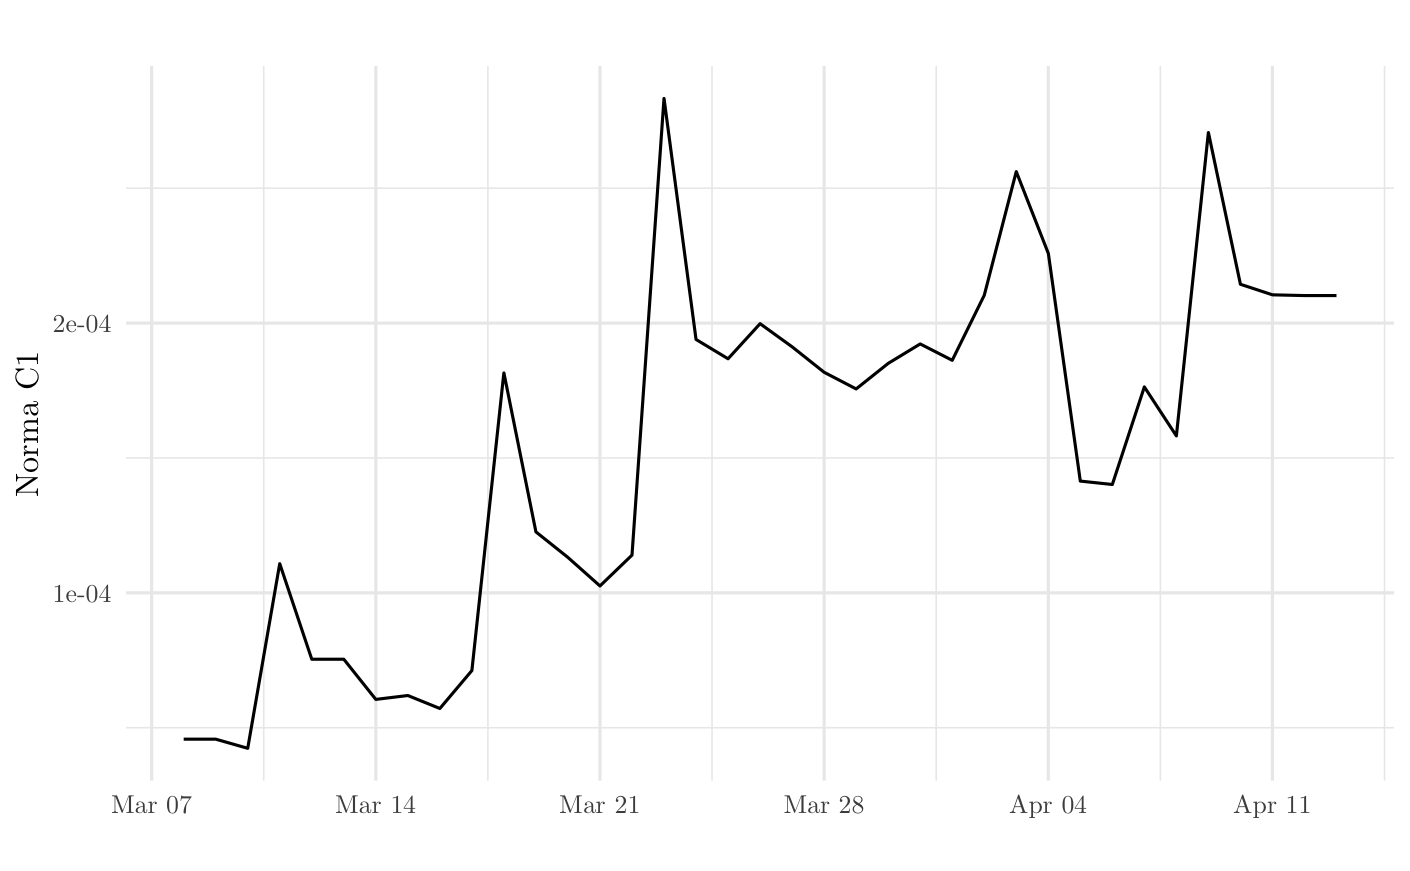
\includegraphics[scale=0.3]{Chapter5/norma_c1_3meses.png}
	\caption{Norma $C^1$ desde enero hasta abril de 2022}
	\label{fig24}
\end{figure}

\begin{figure}[h!]
	\centering
	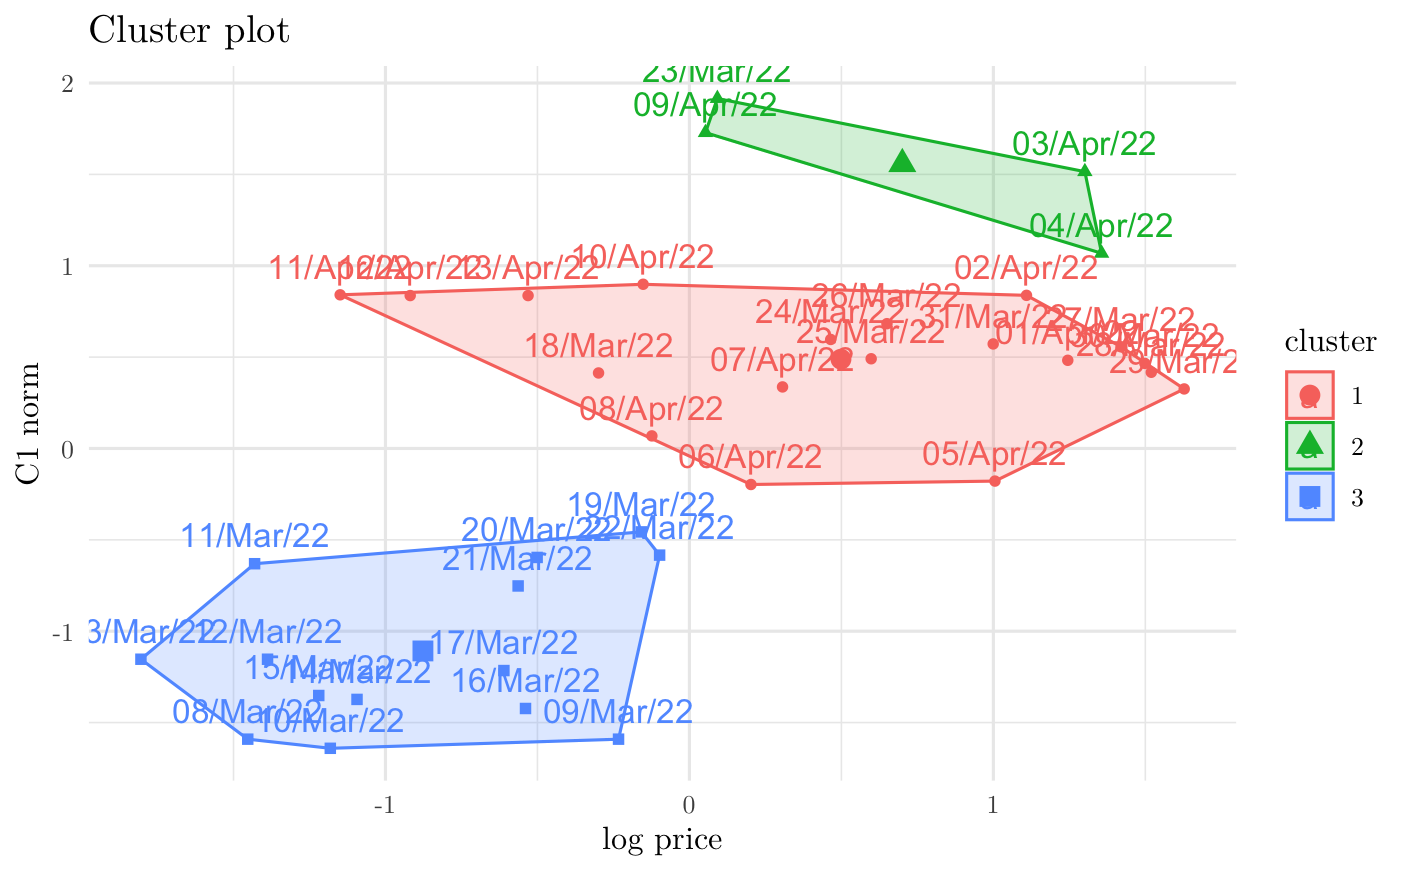
\includegraphics[scale=0.3]{Chapter5/cluster_riesgo.png}
	\caption{Agrupamientos generados usando K-means para detectar el cluster de riesgo de caídas}
	\label{fig25}
\end{figure}

\begin{figure}[h!]
	\centering
	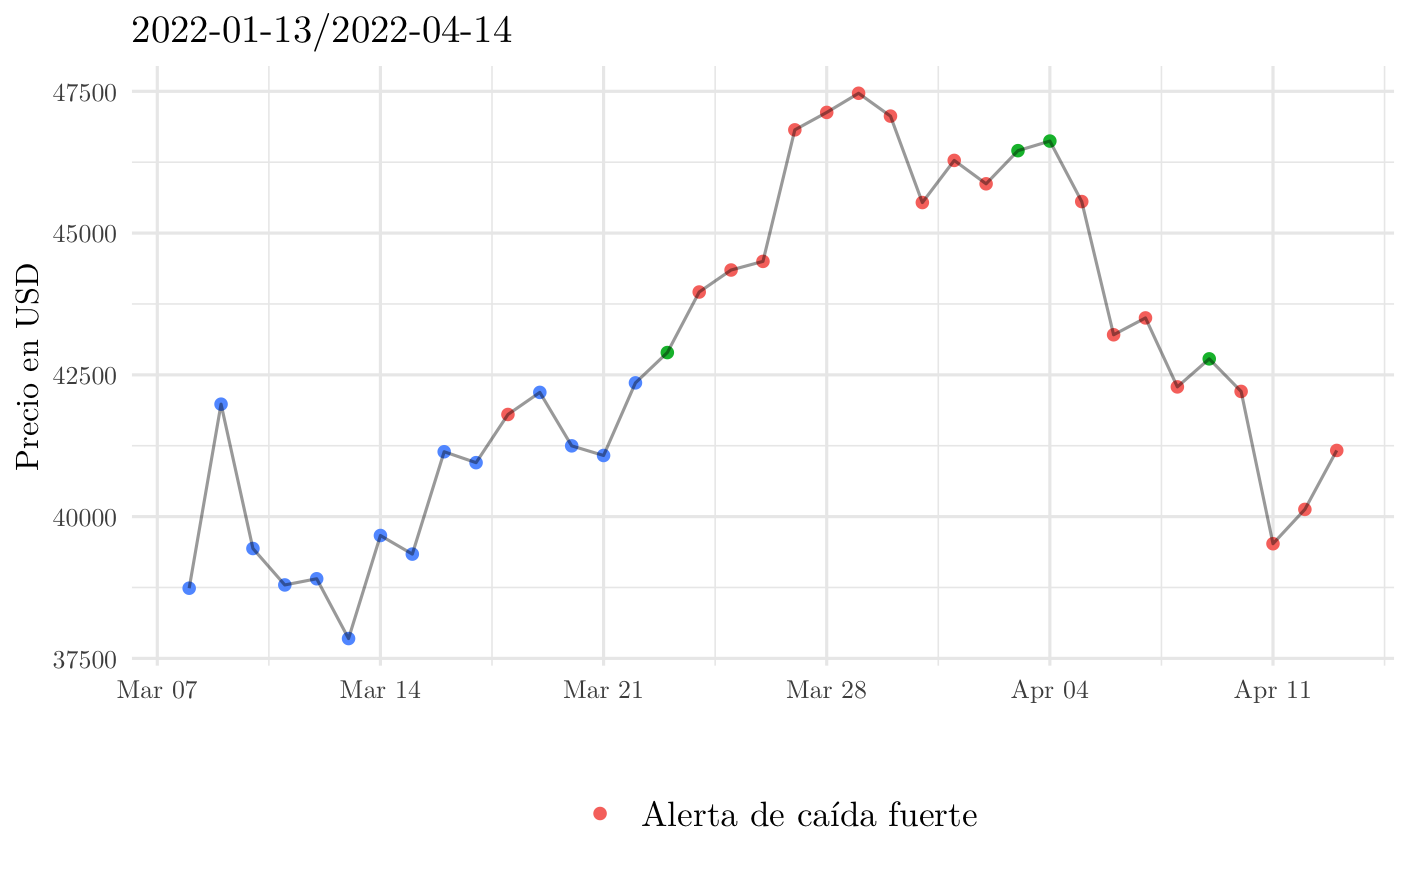
\includegraphics[scale=0.3]{Chapter5/pred_TDA.png}
	\caption{Cluster de riesgo sobre datos del precio originales}
	\label{fig26}
\end{figure}


\section{Clasificación}
\label{res_clasificacion}

\subsection{Transformaciones}
Ya que los datos utilizados son los mismos que en la predicción, estos se cargan directamente para ser transformados, la \autoref{fig27} muestra los datos originales, las normas $C^1$ obtenidas anteriormente y los datos transformados por la entropía de Shannon. 

\begin{figure}[h!]
	\centering
	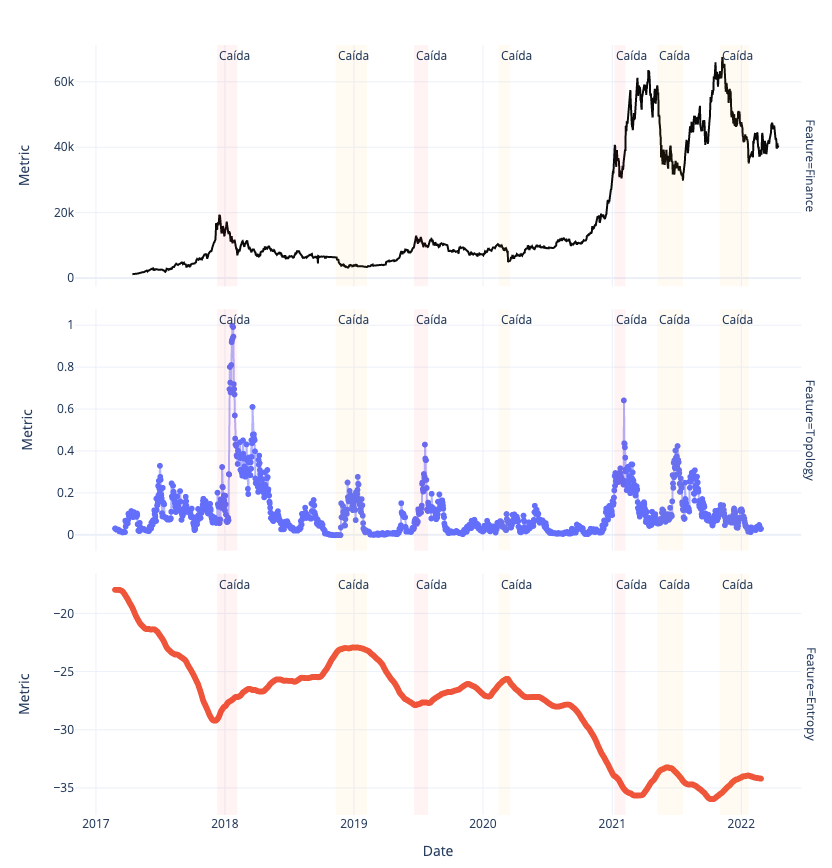
\includegraphics[scale=0.55]{Chapter5/clasifica_transf.png}
	\caption{Características obtenidas de la entropía y el análisis topológico y su relación con las caídas del precio}
	\label{fig27}
\end{figure}
\vspace{1cm}
Como se puede observar en las caídas en rojo, el análisis topológico de datos nos ayuda a prever caídas significativas después de un crecimiento constante en periodos cortos de tiempo. Entre mayor sea la norma $C^1$ mayor será la caída después del aumento del precio. Como se muestra en el crac del 2018, en una semana el precio bajo un 26\% con respecto al actual. A mediados del 2019 el precio sufrió una caída aproximada del 25\% en 7 días mostrando una característica topológica igualmente alta. Por otro lado, a inicios de 2021, del 14 de enero al 21 de enero hubo una caída significativa del 29\% en 7 días. Si se nota la entropía calculada, ésta caracteriza las bajadas del precio con un pequeño valle en la serie de tiempo.

Si la caída ocurre mientras el precio se mantiene relativamente constante o en un periodo largo de tiempo como en los periodos de 2019, 2020, 2021 y 2022 (caídas en naranja) la norma $C^1$ muestra un aumento pero no de forma significativa. La entropía captura mesetas en estos periodos de tiempo que entre más pronunciadas, mayor es la norma $C^1$.
\subsection{Selección de cluster de inversión}

Con las características anteriores se crea un plano que tiene por eje $x$ la entropía normalizada y en el eje $y$ la norma $C^1$ igualmente normalizada. Se agrupan los puntos con el algoritmo K-means de tal forma que estos nos ayuden a detectar las subidas y bajadas del precio para caracterizar la toma de decisiones de inversión como se observa en la \autoref{fig28}.

\begin{figure}[h!]
	\centering
	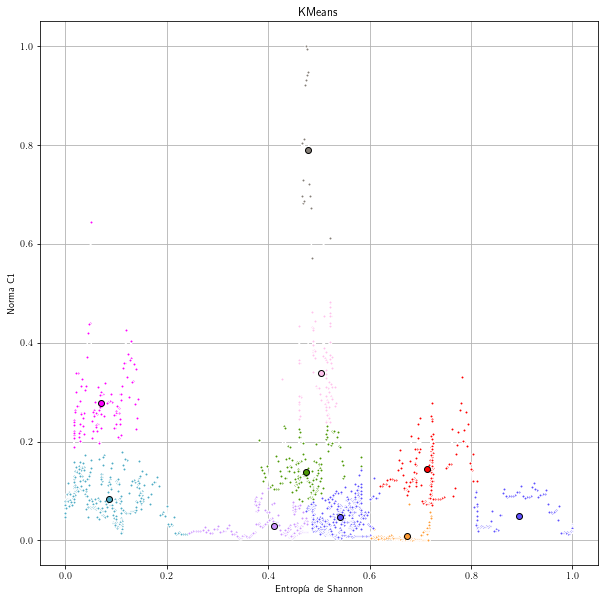
\includegraphics[scale=0.5]{Chapter5/calsifica_kmeans.png}
	\caption{Clusters generados a partir de la entropía y la norma $C^1$ para la toma de decisiones de inversión}
	\label{fig28}
\end{figure}

Estos agrupamientos son llevados a los datos originales donde se lleva a cabo la selección manual de los clusters de comprar, vender o arriesgar. Cuando el precio baja (o hay una caída) se recomienda comprar, cuando sube se recomienda vender

\begin{figure}[h!]
	\centering
	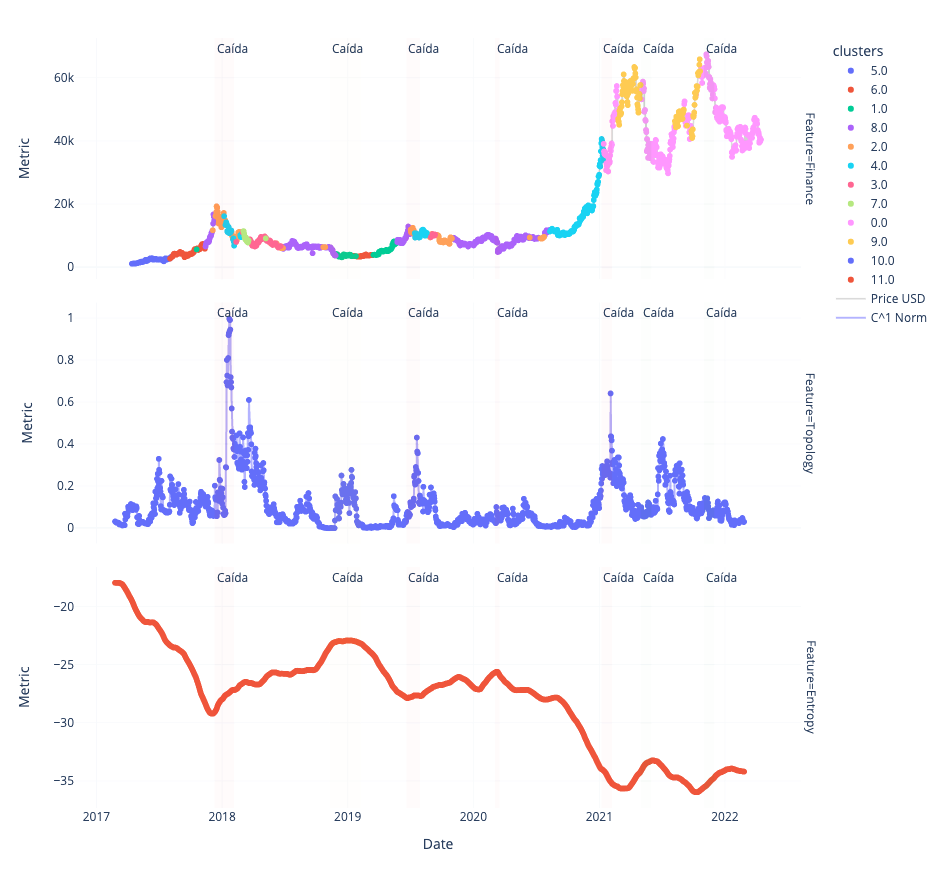
\includegraphics[scale=0.5]{Chapter5/clasifica_inv2.png}
	\caption{Clusters sobre datos del precio originales para la elección manual de los agrupamientos de inversión}
	\label{fig29}
\end{figure}

Los agrupamientos seleccionados para comprar fueron: 2,3,7,0, para vender: 4,5,6,8,9, y arriesgar: 1.
Las imagenes generadas a partir de los datos originales y sus respectivos agrupamientos se muestran en la \autoref{fig30}. 

\begin{figure}[h!]
	\centering
	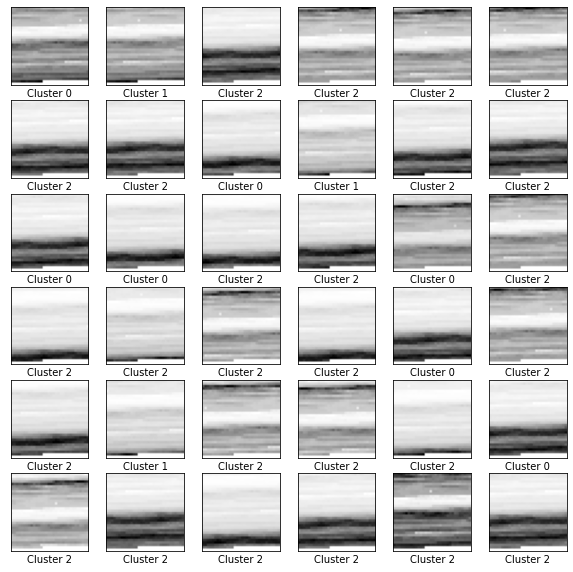
\includegraphics[scale=0.5]{Chapter5/IMG_cluster.png}
	\caption{Imágenes generadas a partir de la serie de tiempo}
	\label{fig30}
\end{figure}

\subsection{Modelo de clasificación}

Despues del entrenamiento con el 80\% de los datos se alcanza una exactitud del 95.76\% sobre los datos de entrenamiento como se observa en la \autoref{fig31}.

\begin{figure}[h!]
	\centering
	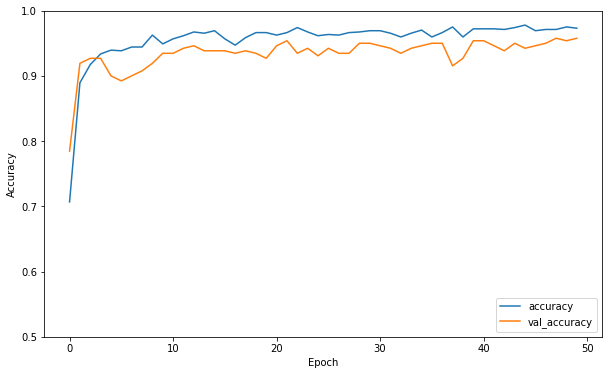
\includegraphics[scale=0.6]{Chapter5/exactitud_clas.png}
	\caption{Exactitud sobre el conjunto de entrenamiento (azul) y el conjunto de prueba (naranja)}
	\label{fig31}
\end{figure}

El modelo es guardado y cargado para realizar predicciones sobre intervalos mayores a 32 días, de tal forma que se realiza una recomendación de inversión utilizando el color rojo para vender, el verde para comprar y el naranja para arriesgar. La linea punteada en la \autoref{fig32} muestran los promedios móviles de 30 días sobre los datos para ayudar a entender mejor la recomendación de inversión. 

\begin{figure}[h!]
	\centering
	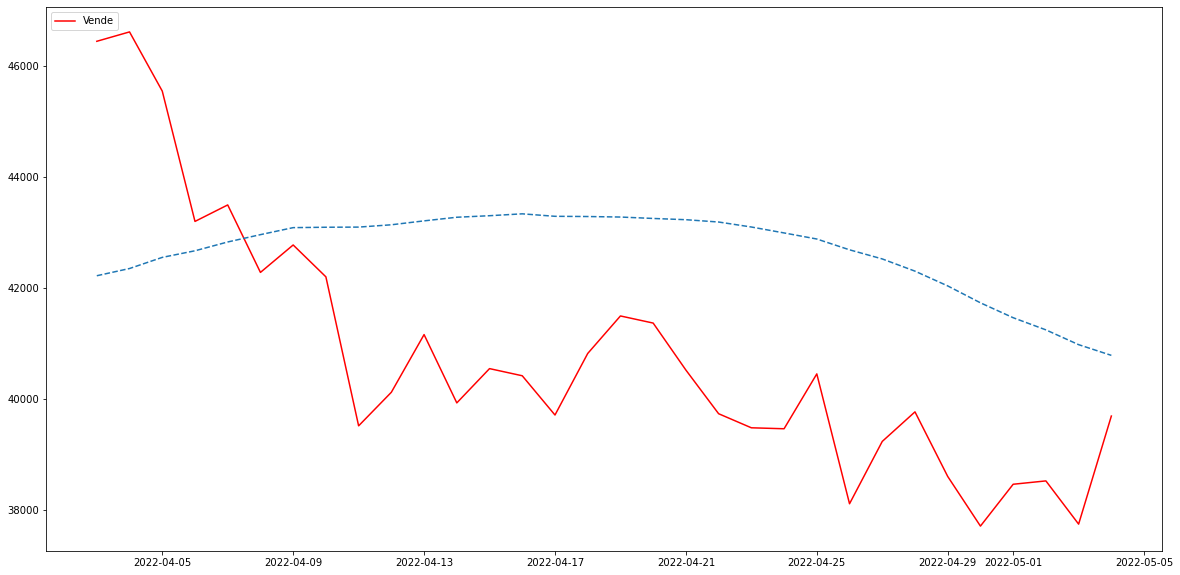
\includegraphics[scale=0.4]{Chapter5/reco.png}
	\caption{Recomendación de inversión del mes de abril a mayo de 2022}
	\label{fig32}
\end{figure}

\begin{figure}[h!]
	\centering
	\subfloat[Crac del 2018]
	{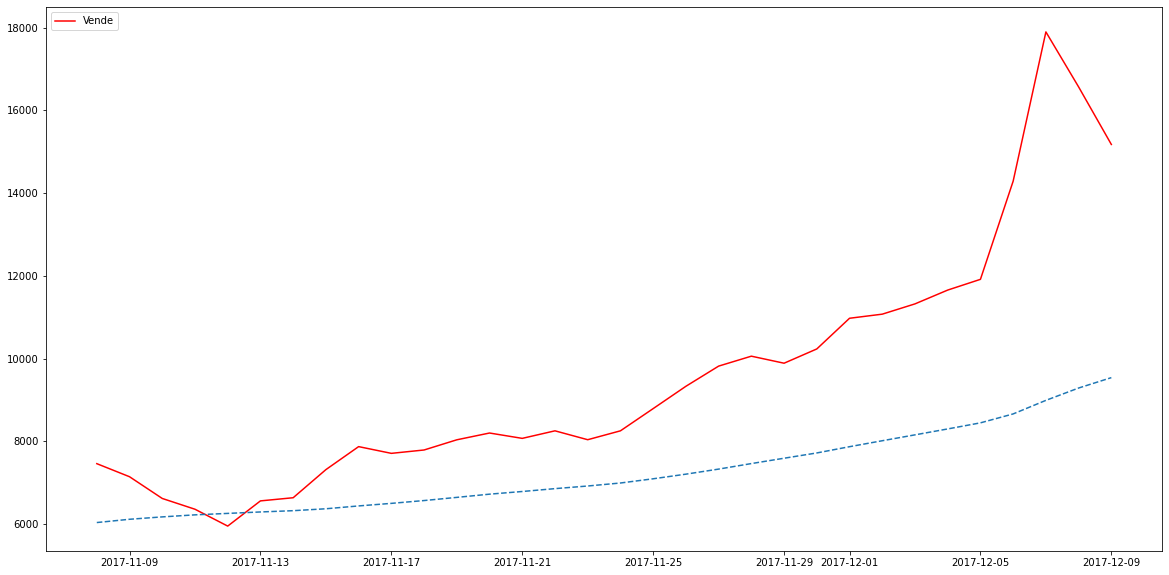
\includegraphics[width=0.47\columnwidth]{Chapter5/2018_crac_vende.png}}
	\qquad
	\subfloat[Mínimos despues del crac del 2018]
	{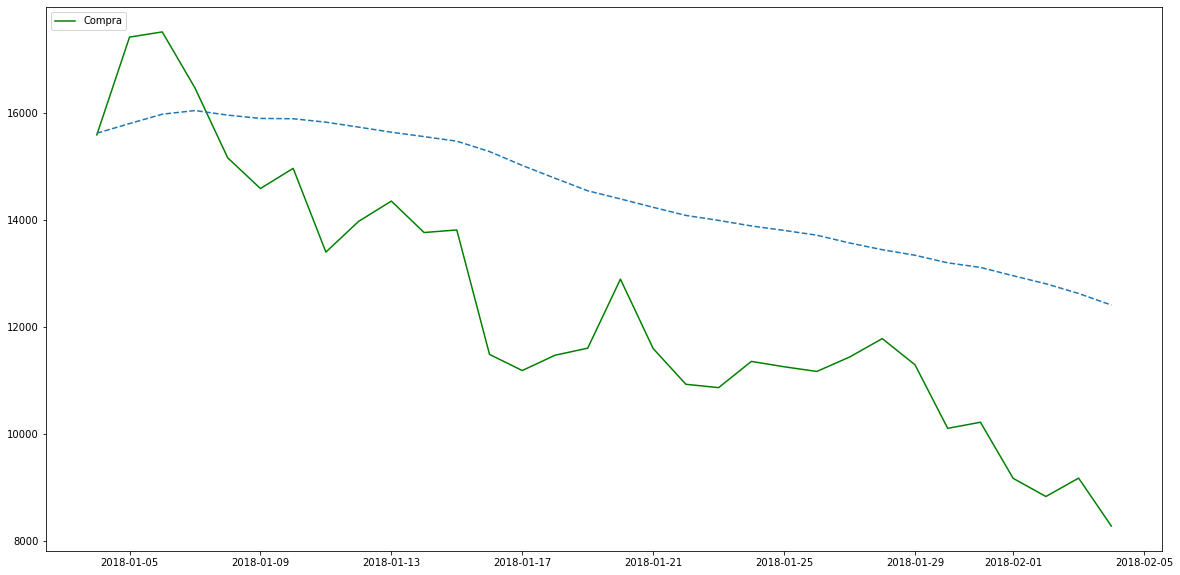
\includegraphics[width=0.47\columnwidth]{Chapter5/2018_crac_compra.png}}
	\qquad
	\subfloat[Crac del mediados del 2021]
	{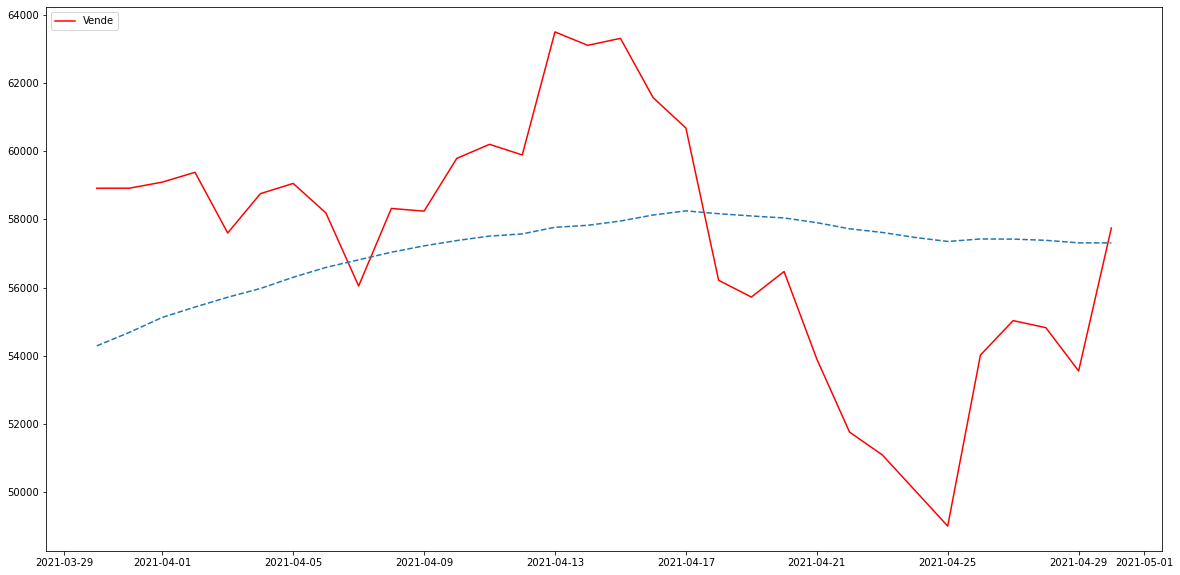
\includegraphics[width=0.47\columnwidth]{Chapter5/2021_crac_vende.png}}
	\qquad
	\subfloat[Mínimos despues del crac del 2021]
	{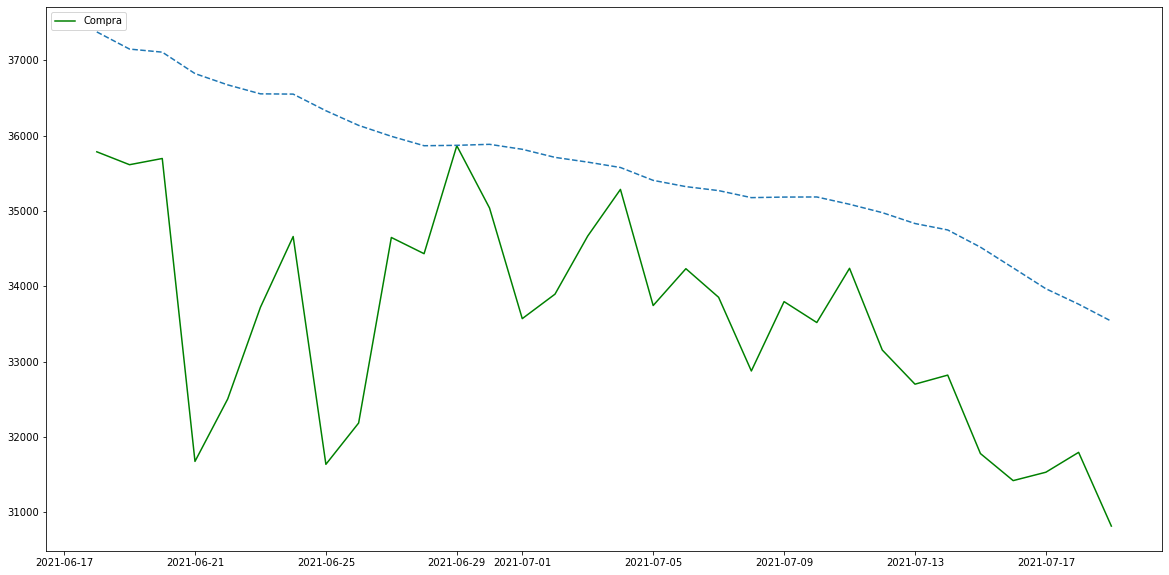
\includegraphics[width=0.47\columnwidth]{Chapter5/2021_crac_compra.png}}
	
	\caption{Recomendaciones de inversión en los intervalos de caídas criticas del precio.}
	\label{fig33}
\end{figure}

En este caso, en un intervalo del cinco de abril al cinco de mayo de 2022, el algoritmo recomienda vender, ocurriendo en los tres días siguientes una caída desde \$39,700 dólares a \$34,500 dólares.

En las caídas drásticas de periodos anteriores  también se realiza una correcta predicción como se muestra en la \autoref{fig33}. Se llega a predecir correctamente y con anticipación el crac de 2018 y 2021 con sus respectivos precios mínimos después de las caídas ayudando a tomar la decisión de realizar una compra.
